%% Template for ENG 401 reports
%% by Robin Turner
%% Adapted from the IEEE peer review template

%
% note that the "draftcls" or "draftclsnofoot", not "draft", option
% should be used if it is desired that the figures are to be displayed in
% draft mode.

% \documentclass[peerreview,onecolumn]{IEEEtran}

\documentclass[11pt,a4paper]{article}

% Set margins
\usepackage[a4paper, margin=1in]{geometry}

\usepackage{cite} % Tidies up citation numbers.
\usepackage{url} % Provides better formatting of URLs.
\usepackage[utf8]{inputenc} % Allows Turkish characters.
\usepackage{booktabs} % Allows the use of \toprule, \midrule and \bottomrule in tables for horizontal lines
% Required packages
\usepackage{graphicx}   % For including images
\usepackage{float}      % For precise float positioning with [H]
\usepackage{amsmath}    % For mathematical symbols and equations
\usepackage{hyperref}   % For hyperlinks
\usepackage{subcaption} % For subfigures and captions
\usepackage{ragged2e}   % for justifying

\usepackage{amsfonts}

\usepackage{braket}
\usepackage{listings}

\usepackage{amsmath}


\title{Introduction to Quantum Machine Learning}
\begin{document}


\author{Sushant Padha \\
Computational Physics Project 2024\\
Indian Institute of Technology, Bombay\\
}
\date{18/1/24}

% make the title area
\maketitle
\tableofcontents
\listoffigures
% \listoftables

\newpage
\begin{abstract}
This report explores the field of quantum computing starting with introductory notions and extending it via techniques based on variational quantum algorithms (VQAs) and differentiable quantum circuits (DQCs), to solve foundational problems. Introductory quantum mechanical theory is introduced along with quantum algorithm design and applied to a quantum teleportation circuit. Results obtained from simulations and IBMQ hardware execution are compared to highlight the scope for applying theory to practice using current era noisy intermediate-scale quantum (NISQ) devices. The variational quantum eigensolver (VQE) is used to compute ground state energies, demonstrating efficient optimization on noisy intermediate-scale quantum (NISQ) devices. Additionally, a quantum solver is developed for nonlinear differential equations using rich latent space-based feature maps and hybrid quantum-classical workflows used to solve ordinary differential equations (ODEs) with highly nonlinear solutions. A variation is discussed and implemented, emphasizing the utility of physics-informed neural networks, in order to solve the 2D Laplace equation. The findings underscore the promise of current quantum technologies in tackling computationally intensive problems, with insights for future integration on practical quantum devices. 

\end{abstract}

\section{Introduction}
Quantum mechanics forms the foundation of quantum computing, which leverages principles such as superposition, entanglement, and quantum interference to solve problems that are infeasible for classical computation. Unlike classical computers that process information in binary bits, quantum computers use qubits, which can represent and manipulate information in superposition states. This allows quantum systems to process exponentially larger amounts of data in certain scenarios.

Variational quantum algorithms (VQAs) represent a promising class of algorithms designed for noisy intermediate-scale quantum (NISQ) devices. These algorithms employ hybrid quantum-classical workflows, where a quantum processor handles the preparation of quantum states and a classical processor optimizes the parameters iteratively. VQAs are particularly advantageous for problems like optimization, quantum chemistry, and machine learning, offering a pathway to achieve quantum advantage in the near term.

Quantum computing offers several key speedups over classical methods:

\begin{enumerate}
    \item Exponential scaling of state space: The state space of a quantum system scales exponentially with the number of quantum components (or qubits) allowing us to explore feature spaces that are infeasible to represent classically.
    \item Quantum algorithms: They utilize concepts such as superposition, entanglement and quantum interference which offer superpolynomial or even exponential speedups compared to classical counterparts (for e.g. Shor's algorithm for factorization).
    \item Simulation of quantum systems: Classical methods struggle with the exponential complexity of simulating quantum systems, but quantum computers excel in this domain using algorithms like the variational quantum eigensolver (VQE).
\end{enumerate}

This project explores these paradigms through two implementations: the variational quantum eigensolver (VQE) \cite{VQA} for finding ground state energies and a nonlinear differential equation solver using differentiable quantum circuits (DQCs) \cite{DQC}. Additionally, as part of foundational learning, a quantum teleportation circuit was implemented to illustrate core concepts of entanglement and quantum operations.
  

\section{Introduction to Quantum Mechanics and Quantum Computing}

\subsection{Basic notions}

The fundamental unit of information in quantum computing is a qubit which, unlike classical bits that only exist in either a $0$ or $1$ state, can exist in a superposition, or linear combination of multiple states, a concept which is unique to quantum computing.

A qubit is said to exist in a Hilbert space, an abstract vector space equipped with an inner product, which is the general characteristic of the state space of any quantum system. One common representation of qubits is as a superposition of basis states, here $\ket{0}, \ket{1}$ respectively, collectively referred to as the "computational basis".

$$\ket{\psi} = \alpha\ket{0} + \beta\ket{1}$$ \\
where the state is normalized as $|\alpha|^2 + |\beta|^2 = 1$, for some complex amplitudes $\alpha$ and $\beta$.

The evolution of a quantum system is represented as a series of unitary transformations. Mathematically, they can be expressed as linear operators with real eigenvalues, that is, Hermitian, that preserve norm with respect to the inner product defined on the vector spaces acted on and produced by it.

Qubits are evolved by applying "quantum gates" which are loosely comprised of unitary operators and measurement operators. Unitary operators may be single qubit like the Pauli operators $\hat{I}, \hat{\sigma_x}, \hat{\sigma_y}, \hat{\sigma_z}$, or multi-qubit such as \texttt{CNOT}, etc.

Composite systems can be described as tensor product of individual states. A key idea of \textbf{entanglement} is relevant here, as some composite states cannot be represented as a product of simpler states, the most famous example being the typical Bell state
$$\ket{\Psi^+} = \frac{\ket{00} + \ket{11}}{\sqrt{2}}$$
It represents a two-qubit state that exists as $\ket{00}$ and $\ket{11}$ which $1/2$ probability each, hence, measuring any one qubit in some state will cause the other to immediately to collapse to the same state, an idea that is utilized in many quantum algorithms.

The quantum circuit model is used to describe algorithms on qubits and measure the results. It is composed of wires or "quantum register", representing qubits moving through time and acted upon by various operators, before being measured (or not, in the case of ancillary qubits).

\subsection{Quantum Teleporation Algorithm}

One of the most intriguing applications of quantum mechanics is quantum teleportation, a protocol to transmit an unknown quantum state between two distant parties using entanglement and classical communication. The key steps of the algorithm are:

\begin{enumerate}
    \item Alice has a qubit whose quantum state $\ket{\psi} = \alpha\ket{0} + \beta\ket{1}$ she wants to send to Bob
    \item First, an entangled Bell pair such as $\ket{\beta_{00}} = \frac{\ket{00} + \ket{11}}{\sqrt{2}}$ is created and shared between Alice and Bob
    \item The initial state of the system is the tensor product of Alice's unknown qubit with the Bell state $\ket{\psi_0} = \ket{\psi}\ket{\beta_{00}}$
    \item Alice performs a \texttt{CNOT} gate operation on her qubits, using the unknown qubit as the control and her share of the Bell pair as the target and then applies a Hadamard gate to the unknown qubit
    \item Alice measures both of her qubits in the computational basis and obtains a classical two-bit result. She then sends this result to Bob via a classical communication channel
    \item Bob applies a single-qubit operation conditioned on the two bits received from Alice. If the result is $00$, Bob’s qubit is already in state $\ket{\psi}$, if it is $01$, he applies $X$; if it is $10$, he applies $Z$; and if it is $11$, he applies $ZX$
    \item After Bob applies the operation, the quantum state of his qubit is identical to Alice's original qubit $\ket{\psi}$
\end{enumerate}

This process transfers the quantum state of the qubit from Alice to Bob without physically moving the qubit itself and relies on the non-local correlation of entangled states.

\subsubsection{Methodology}

The algorithm is implemented using the Python library, Qiskit. First, we create a quantum circuit object using \texttt{QuantumCircuit} class, filled with a quantum register and correspondingly classical registers of 3 qubits and 3 classical bits each. The first qubit ($q_0$) is prepared in the state we wish to teleport using the \texttt{Statevector} class to generate arbitrary statevector. We take the case of $\alpha = 0.6, \beta = 0.8$, or $[0.6 \quad 0.8]^T$ statevector. Then, we prepare entangled Bell state using qubits two and three ($q2, q3$ resp.). Then, apply \texttt{CNOT} from $q_0$ to $q_1$ followed by Hadamard gate in order to entangle Alice's qubit ($q_0$) with her pair of the Bell state ($q_1$). Finally, we measure Alice's qubits ($q_0, q_1$) and apply the relevant gates to $q_2$ based on the bitstring received. Ultimately, the recieved $q_2$ is sampled many times to estimate its probability distribution and check the algorithm's accuracy.

% The algorithm is implemented as a circuit in Qiskit using the following code:
% \begin{lstlisting}[language=Python]
% ### Setup the circuit
% qbits = QuantumRegister(3, "q")
% clbits = ClassicalRegister(3, "c")
% qc = QuantumCircuit(qbits, clbits)

% ### State to teleported
% # alpha=0.6, beta=0.8 as an example
% psi = Statevector([0.6, 0.8])

% qc.prepare_state(psi, 0)
% qc.barrier()

% ### Prepare bell state
% qc.h(2) # hadamard on q2
% qc.cx(2, 1) # CNOT from q2 to q1
% qc.barrier()

% ### Apply cx and h gates
% qc.cx(0, 1) # CNOT from q0 to q1
% qc.h(0) # hadamard on q0
% qc.barrier()

% ### Measure
% qc.measure(0, 0)
% qc.measure(1, 1)
% qc.barrier()

% ### Apply gates based on measurement
% qc.cz(0, 2)
% qc.cx(1, 2)
% qc.barrier()

% ### Finally measure q2 or sampling
% qc.measure(2, 2)

% # draw circuit
% fig = qc.draw('mpl')
% \end{lstlisting}

\begin{figure}[H]
    \centering
    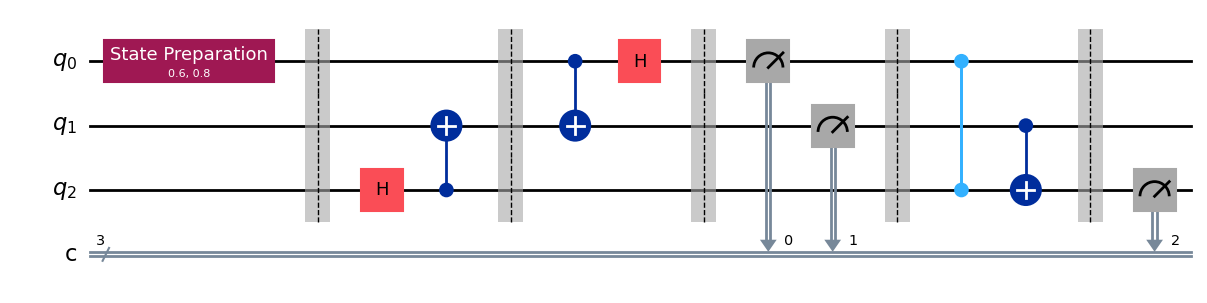
\includegraphics[width=0.8\textwidth]{quantum-teleportation-circuit}
    \caption{Visual representation of the quantum teleportation circuit}
    \label{fig:quantum-teleportation-circuit}
\end{figure}

Qiskit offers two methods to execute the circuit, using the \texttt{Estimator} and \texttt{Sampler} primitives. Here, we use the latter and sample 4096 shots of the above circuit, on both a local simulator (Aer Sampler) and on real IBM Quantum hardware, accessible via the \texttt{qiskit\_ibm\_runtime} Python library. Here, we run the circuit on the \texttt{ibm\_brisbane} backend.

For running the circuit on either real or simulated hardware, it must decomposed to the gate alphabet of the target hardware, that is, each logical gate must be expressed as a combination of simpler gates that can be physically realized, in a manner that is efficient and mitigates error and decoherence effects as much as possible.

This is done as:
\begin{lstlisting}[language=Python]
# for local simulator
decomposed_circuit = qc.decompose(reps=6)

# for IBM quantum hardware
pm = generate_preset_pass_manager(
    backend=backend, optimization_level=1)
isa_circuit = pm.run(qc)
\end{lstlisting}

The circuit compiled for the IBMQ backend \texttt{ibm\_brisbane} is shown here in \ref{fig:quantum-teleportation-isa-circuit}.

\begin{figure}[H]
    \centering
    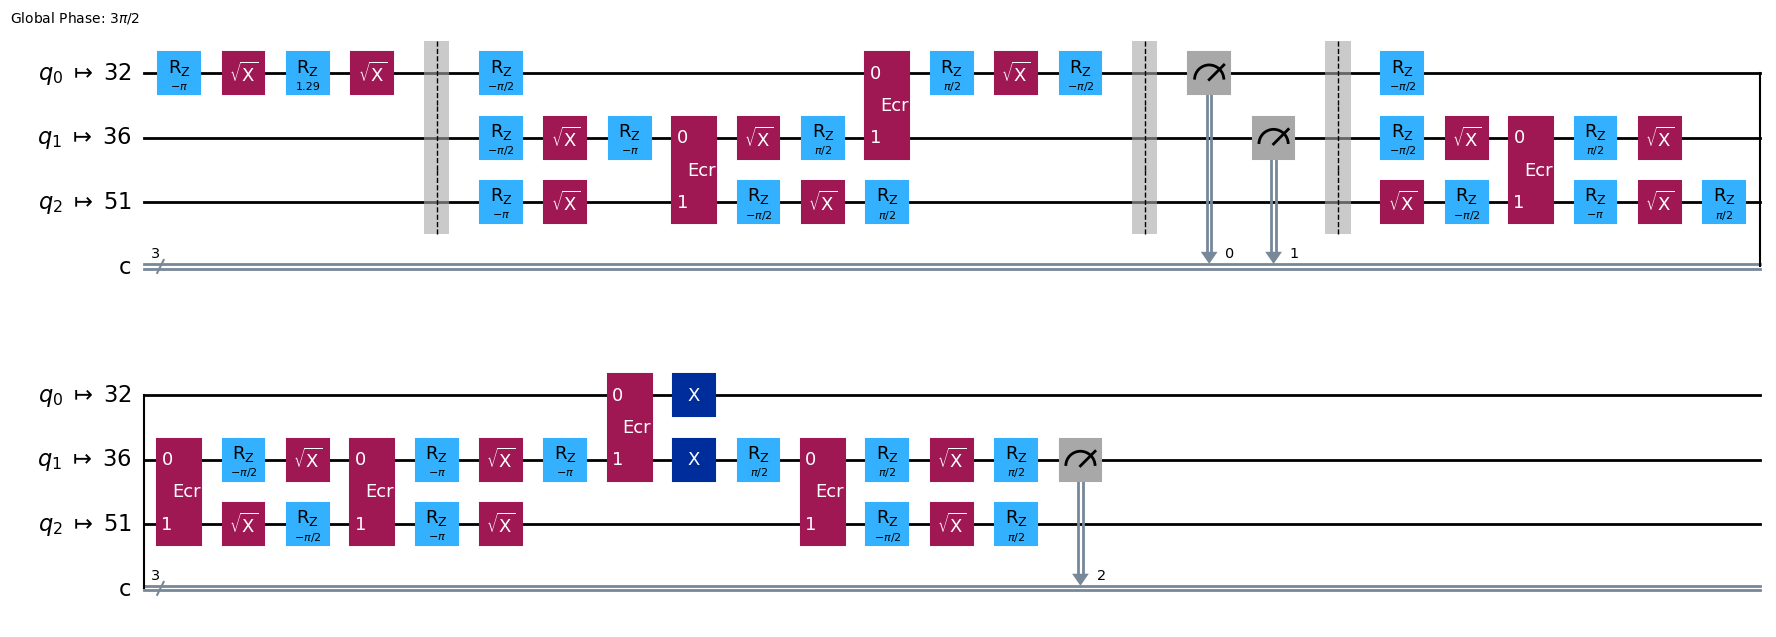
\includegraphics[width=0.8\textwidth]{quantum-teleportation-isa-circuit.png}
    \caption{Visual representation of the compiled circuit}
    \label{fig:quantum-teleportation-isa-circuit}
\end{figure}

\subsection{Results and analysis}

Ideally, the quantum circuit should teleport the state exactly and produce $q_2 = 0.6\ket{0} + 0.8\ket{1}$ in all cases. Hence, we expect the probabilities to be very close to $|\alpha|^2 = 0.36$ and $|\beta|^2 = 0.64$ for measurement $0$, $1$ respectively.

\begin{figure}[H]
    \centering
    % First image
    \begin{subfigure}[t]{0.45\textwidth}
        \centering
        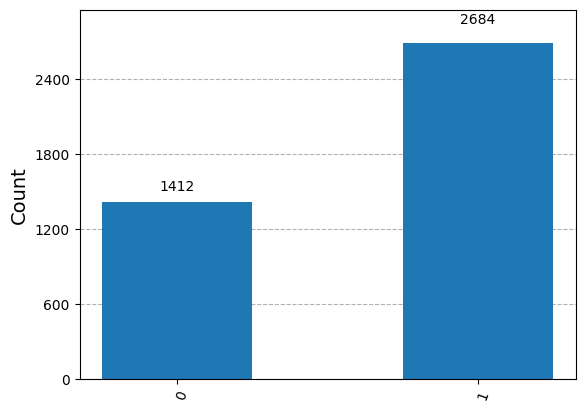
\includegraphics[width=\textwidth]{local-counts.png} % Replace with your image
        \caption{Counts of each state on sampling $q_2$}
        \label{fig:local-counts}
    \end{subfigure}
    \hfill
    % Second image
    \begin{subfigure}[t]{0.45\textwidth}
        \centering
        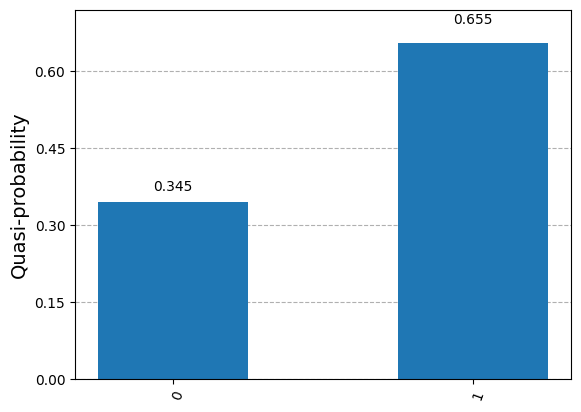
\includegraphics[width=\textwidth]{local-quasiprobabilities.png} % Replace with your image
        \caption{Quasi-probabilities of each state on sampling $q_2$}
        \label{fig:local-quasiprobabilities}
    \end{subfigure}
    \caption{Local Aer simulator results}
    \label{fig:local}
\end{figure}

The number of shots for each state are shown in fig. \ref{fig:local-counts}, and the corresponding quasi-probabilities (calculated as a ratio of the total number of shots) are shown in fig. \ref{fig:local-quasiprobabilities}.

The local Aer simulator based results bear a very close resemblance to the behavior expected from an ideal quantum system being operated on by the algorithm.

Note that the Aer-based local simulator can store the exact statevectors after every unitary gate operation using the \texttt{StatevectorSimulator} implementation. However, it is not being utilized in this case because the circuit involves intermediate step measurements, which cannot be exactly simulated. Still, this does not introduce any error.

When the final measurement is made, the state must collapse to one of the two computational basis states with precisely the probabilities $0.36$ and $0.64$. The slight mismatch in final values may be attributed to a finite number of shots. As we increase number of shots, the results will become more accurate.

\begin{figure}[H]
    \centering
    % First image
    \begin{subfigure}[t]{0.45\textwidth}
        \centering
        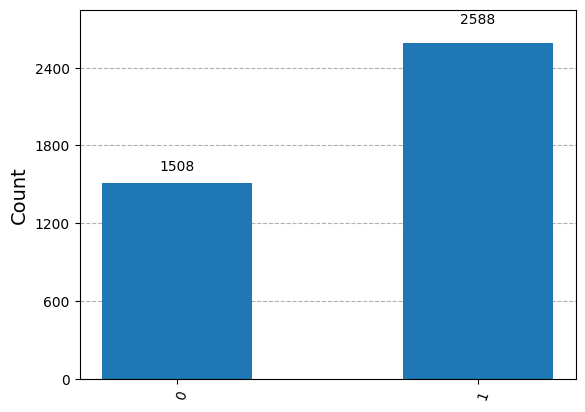
\includegraphics[width=\textwidth]{ibmq-counts.png} % Replace with your image
        \caption{Counts of each state on sampling $q_2$}
        \label{fig:ibmq-counts}
    \end{subfigure}
    \hfill
    % Second image
    \begin{subfigure}[t]{0.45\textwidth}
        \centering
        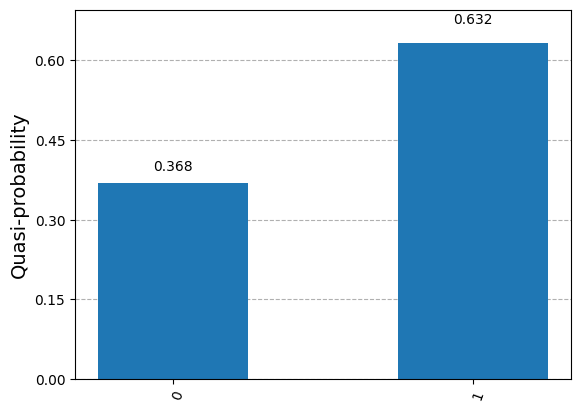
\includegraphics[width=\textwidth]{ibmq-quasiprobabilities.png} % Replace with your image
        \caption{Quasi-probabilities of each state on sampling $q_2$}
        \label{fig:ibmq-quasiprobabilities}
    \end{subfigure}
    \caption{IBMQ hardware results}
    \label{fig:ibmq}
\end{figure}

Results analagous to figures \ref{fig:local-counts} and \ref{fig:local-quasiprobabilities} are shown in figures \ref{fig:ibmq-counts} and \ref{fig:ibmq-quasiprobabilities} for real hardware execution.

The IBMQ hardware execution results also match the expected ratio very well, however with longer execution time.

However, in the case of execution on real quantum hardware, there are many sources of error like error in preparing the initial $\ket{\psi}$ state on the target hardware, gate imperfections, decoherence of the entangled states over the duration of circuit execution and environmental noise.

This introduces additional error in the final $q_2$ state which is not present in Aer-based execution. Finally, we lose some precision due to the finite number of shots.

\subsection{Summary}

To summarize, the foundational concepts of quantum computing were applied by implementing the quantum teleportation algorithm. The results of execution on the IBMQ hardware are close to the expected values. We can tentatively conclude that there is scope of applying present era devices to simple problems solvable via quantum circuits. Circuits with low number of qubits and shallow depth can be executed effectively, with the error rate being well under control.

Reflecting on one of the issues with this implementation, sampling the state is not desirable since the final $q_2$ state may have a change in its phase ($0.6\ket{0} + 0.8 e^{i\varphi} \ket{1}, \; 0 < \varphi < 2\pi$) while keeping probabilities the same. It would be most appropriate to construct an observable in the form of a projector $P = \ket{\psi}\bra{\psi}$ and use the \texttt{Estimator} class to measure its expectation value (values close $+1$ indicate strong correlation). Additionally, we can make use of the \texttt{StatevectorSimulator} by moving all the measurements to the end according to the principle of deferred measurement \cite[p.~186]{nielsen_chuang}, which will likely improve performance.

\section{Variational Quantum Algorithms}

\subsection{Introduction}

Variational Quantum Algorithms (VQAs) represent a powerful hybrid approach that leverages the strengths of both quantum and classical computation. With the present era NISQ devices, VQAs have emerged as the leading strategy to obtain quantum advantage. This class of algorithms is based on the variational principle in quantum mechanics which involves taking a trial wavefunction, parametrized by a finite set of continuous and/or discrete parameters which are then optimized to minimize an expectation value.

VQAs are being considered the quantum analog to the largely successful category of machine learning algorithms or neural networks. They are based on a hybrid quantum-classical workflow to achieve 'quantum supremacy' by evaluating inherently quantum mechanical advised operations such as complex Hamiltonians on the quantum device, and offload the function minimization task (or the corresponding parameter optimization task) to the classical device.

Unlike traditional quantum algorithms that demand fault-tolerant quantum computing, VQAs are well-suited for NISQ hardware due to their shallow circuit depth and noise resilience. This makes VQAs a promising pathway toward achieving quantum advantage in the near term.

\subsection{Basic Tools and Workflow}

\begin{figure}[H]
    \centering
    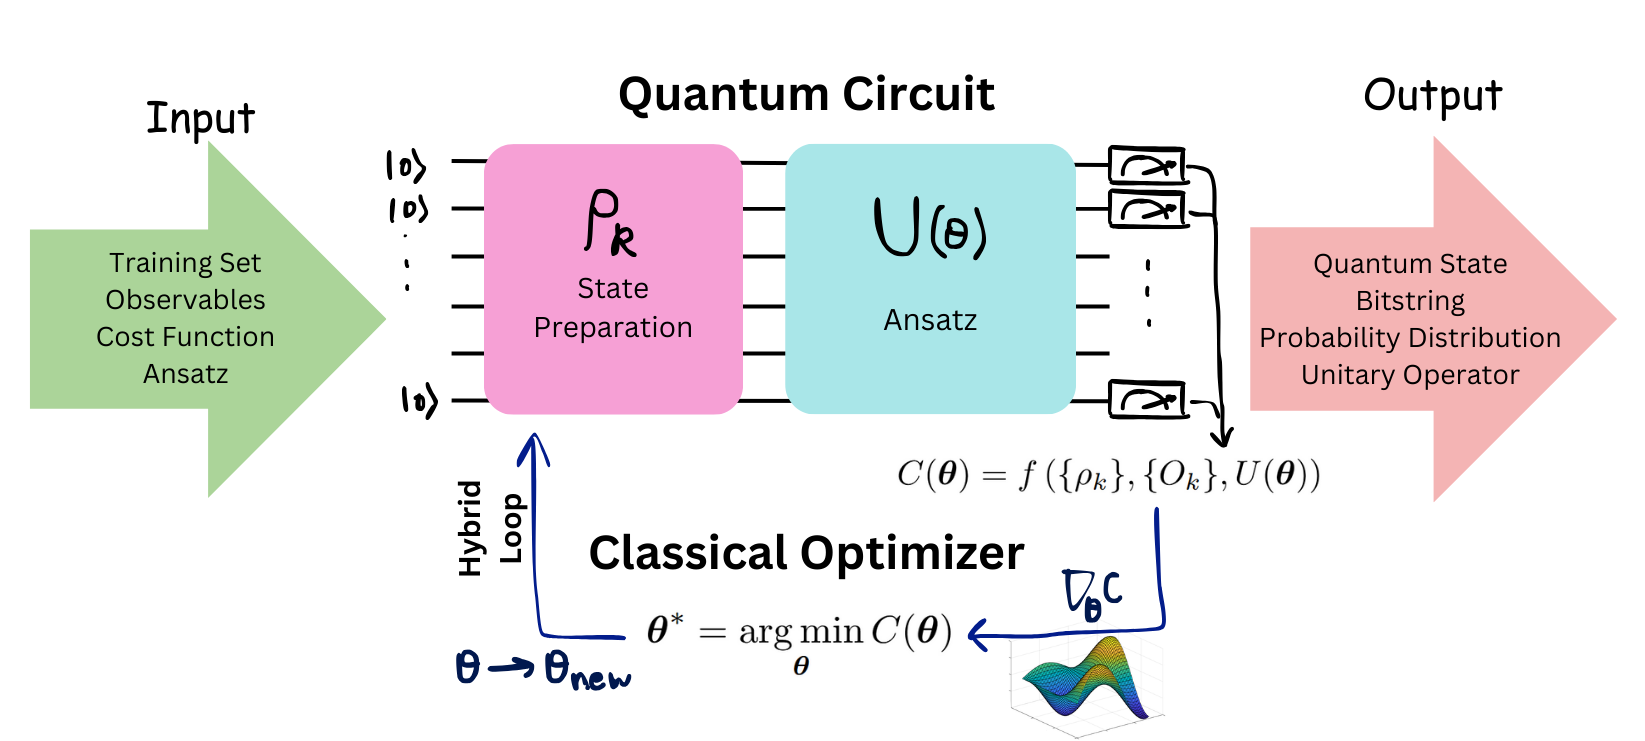
\includegraphics[width=0.8\textwidth]{vqa-schematic.png}
    \caption{Schematic of a variational quantum algorithm (VQA)}
    \label{fig:vqa-schematic}
\end{figure}

We start by considering the problem at hand and modelling a description of that problem and preparing training data, if possible. VQAs can be used to solve a wide variety of problems.

\subsubsection{Cost function}

First, we describe a cost function $C$ which encodes the solution to the problem. This is analagous to the "loss function" used in training neural networks for machine learning. It is desirable that the function can be estimated efficiently (implicitly, more so than on classical computers) on modern day quantum hardware, and that the minimum corresponds to the solution of the problem. It should be easy to optimize, with smaller values correlating with better solutions.

\subsubsection{Other inputs}

Further, we specify a set of training data, or "initial states" that can be fed into the training loop to improve accuracy. A set of observables is mentioned, a linear combination of which can be used for evaluating the cost function.

\subsubsection{Ansatz} \label{sec:Ansatz}

One then proposes an ansatz, that is a parametrized quantum circuit described a set of continuous and/or discrete parameters $\boldsymbol{\theta}$. It is represented as a unitary $\mathcal{\hat{U}}(\boldsymbol{\theta})$ that can be decomposed as product of unitaries, parametrized by $\boldsymbol{\theta}$. The hardware efficient ansatz (HEA) and alternating blocks ansatz (ABA) are well-known examples of 'problem-agnostic' ansatzes. 'Problem-inspired' ansatzes like unitary couples clustered (UCC) ansatz are also used. The quality of an ansatz is gauged in terms of its expressibility and its entangling capability. An ansatz is considered expressible if it can uniformly explore the entire relevant subspace of its solution set.

\subsubsection{Gradient calculation}

Further, the ansatz is trained in a hybrid quantum-classical loop to solve the optimization problem:

$$\boldsymbol{\theta}^* = \arg\min_{\boldsymbol{\theta}} C(\boldsymbol{\theta})$$

This requires efficient computation of the gradient of the cost function. One of the key benefits of using VQAs is that one can evaluate gradients analytically using the parameter shift rule. Unlike numerical differentiation methods like finite differences method, this rule can evaluate the gradient exactly, owing to the periodicity of the gates involved. It can be summarized in vector notation as:

$$
  \nabla C(\boldsymbol{\theta}) = \sum_{i} \frac{\partial C}{\partial \theta_i} \hat{e_i} = \frac{1}{2 \sin(\alpha)} \sum_{i} C(\boldsymbol{\theta} + \alpha \hat{e_i}) - C(\boldsymbol{\theta} - \alpha \hat{e_i})
$$

with $\boldsymbol{e_i}$ being the unit vector in direction of $\theta_i$, being shifted by an amount $\alpha$. The choice of $\alpha = \frac{\pi}{2}$ maximizes accuracy.

Higher order derivatives can be evaluated similarly by applying the rule again, as per the chain rule.

\subsubsection{Optimizer}

The next step is using a classical optimizer that, after estimating the cost function and its gradient from the quantum circuit, processes the results and updates the parameters based on a given optimization schedule. Apart from the standard classical optimization problems, there are additional issues like the inherently stochastic environment due to finite compute resources, hardware noise, problem of barren plateaus. We apply the most common approach, which is based on stochastic gradient descent (SGD). The Adam optimizer is preferred, which adaptively scales the descent steps taken to arrive at the global minima faster. Another approach is to vary the number of shots taken at each step, a frugal approach keeping in mind the capacity of present hardware. Other techniques have also been reviewed in \cite{VQA}.

\subsubsection{Applications}

VQAs can be used to tackle a variety of different tasks. The best-known application of VQAs is to find the ground and excited states of molecular systems, solved using a setup referred to as a variational quantum eigensolver (implementation is detailed in next section). Given a Hamiltonian $\hat{H}$, it produces an approximated ground state $\ket{\Tilde{\psi_G}}$, parametrized by a set of optimized parameters $\boldsymbol{\theta^*}$ as $\ket{\Tilde{\psi_G}} =\mathcal{\hat{U}}(\boldsymbol{\theta^*}) \ket{\psi_0}$.

There are various more specialized applications of this solver. Once an approximated ground state has been obtained, one can use it to find excited states by adding an orthonormal term $a\ket{\Tilde{\psi_G}}\bra{\Tilde{\psi_G}}$ to the Hamiltonian (with $a$ being a positive constant much larger than the energy gap between ground state and first excited state). Other alternatives are also discussed in \cite{VQA}.

Another highly promising potential application is a nonlinear differential equation solver using differentiable quantum circuits \cite{DQC} which is discussed in \ref{sec:DQC}.

\subsubsection{Challenges and potential solutions}

\begin{enumerate}
    \item \textbf{Barren plateaus:} As the number of qubits/depth is increased the error surface becomes increasingly complex which can lead to "barren plateaus" where gradients vanish which are hard to navigate for gradient descent based optimizers. This can be prevented by initializing parameters with small but non-zero values.
    \item \textbf{Commuting operators:} It is noted that the choice of cost function $\mathcal{\hat{C}}$ must be such that it is non-commuting with the circuit unitary  $\mathcal{\hat{U}}$ so that the entire solution space can be spanned. That is, $[\mathcal{\hat{C}}, \mathcal{\hat{G}}] \neq 0$.
    \item \textbf{Effect of noise:} Here, we mostly deal with local statevector simulators but when executing on real hardware, error mitigation must be implemented.
\end{enumerate}

\subsection{Variational Quantum Eigensolver (VQE)}

The problem tackled by a variational quantum eigensolver (VQE) is to find the ground and excited states of molecular systems. First, we describe the system in terms of a Hamiltonian and whose low-lying eigenstates and eigenvalues are to be estimated using variational circuits. We define a cost function as $C(\boldsymbol{\theta}) = \bra{\psi(\boldsymbol{\theta})}\hat{H}\ket{\psi(\boldsymbol{\theta})}$, where $\hat{H}$ is the Hamiltonian operator and $E_G$ is the ground state energy. The aim is to minimize the expectation value of $\hat{H}$ over the trial state $\ket{\psi(\boldsymbol{\theta})} = \mathcal{\hat{U}}(\boldsymbol{\theta})\ket{\psi_0}$. According to the Rayleigh-Ritz variational principle, $C(\boldsymbol{\theta}) \geq E_G$ with the equality holding if $\ket{\psi(\boldsymbol{\theta})}$ is the ground state $\ket{\psi_G}$ of $H$. In practice, the Hamiltonian is represented as a linear combination of product of Pauli operator strings as $\hat{H} = \sum_{a} w_a \hat{P_a}$, where $\hat{P_a} \in \{\hat{I}, \hat{X}, \hat{Y}, \hat{Z}\}^{\otimes N}$, $w_a \in \mathbb{R}$. Since, practically most systems are described by sparse Hamiltonians, the cost function can efficiently estimated with a computational cost that grows at most polynomially with system size, offering major speedup over classical simulation.

\subsubsection{Methodology}

This method explores a basic implementation of a VQE for the 2-qubit state with the Hamiltonian described as $\hat{H} = \hat{X}_0 \hat{X}_1 + \hat{Y}_0 \hat{Y}_1 + \hat{Z}_0 \hat{I}_1$, with $\hat{X}_j, \hat{Y}_j, \hat{Z}_j$ being the Pauli X, Y and Z operators being applied to the $j$-th qubit respectively. The input states are chosen to be comprise simply the all-zeros computational basis state $\ket{0}^{\otimes 2}$, and no other training data is fed in. The cost function is simply defined as the expectation value of the Hamiltonian, which is the target function we wish to minimize. The 'hardware-efficient ansatz' is used, with rotation gates $R_y, R_z$ followed by sets of \texttt{CNOT} gates to entangle neighbouring qubits, repeated for several layers. This is inspired by the 'problem-agnostic' design mentioned earlier, and is easier to train and expressible enough to span the entire subspace for this problem. The variational parameters are the continuous angle parameters in the rotation gates, which are trained in the hybrid loop. Simple stochastic gradient descent is used with a constant learning rate, which can be fine tuned to get the fastest descent while maintaining consistency in final results. Additionally, we explore varying the hyperparameters to determine the optimal set thereof.

The main training loop may be summarized using Qiskit code, as (assume subroutines are suitably defined):

\begin{lstlisting}[language=Python]
# Define observable and hyper-parameters
H = SparsePauliOp(["XX", "YY", "IZ"])
n_qubits = 2
n_layers = 4
alpha = np.pi / 2
eta = 1

# Initialize circuit and parameters
ansatz, n = parameterized_ansatz(n_qubits, n_layers)
th = initialize_parameters(n)

# transpile circuit and transform observable
ansatz_isa = pm.run(ansatz)
H = H.apply_layout(layout=ansatz_isa.layout)

# Training loop
for step in range(steps):
    # Evaluate the cost function
    cost = cost_fn(th)
    
    # Calculate gradients with respect to parameters
    gradients = calculate_gradients(cost_fn, th, alpha)
    
    # Update parameters using gradient descent
    th = update_parameters(th, gradients, eta)
    
# Finalize results
trained_params = th
optimized_circuit = ansatz.assign_parameters(th)
gs = Statevector(optimized_circuit).data
gs_energy = expectation(ansatz_isa, H, estimator, th)
\end{lstlisting}

\subsection{Results and Analysis}

Taking the problem and ansatz structure described in the previous section, we solve it for $N = 100$ iterations, with circuit depth of $d=4$. Rest of the hyperparameters chosen suitably. This circuit is run using the \texttt{AerSimulator} backend and the \texttt{EstimatorV2} primitive is used to estimate the observable values.

We present a metric called the "infidelity" of the quantum state $\ket{\Tilde{\psi_{G}}}$ produced by the unitary evolution corresponding to the trained circuit, as $1 - | \langle\psi_G|\Tilde{\psi_{G}}\rangle|^2$.

To prevent clutter a sampling interval of 5 is used for plotting on the graph.

\begin{figure}[H]
    \centering
    \makebox[\textwidth]{
        \begin{subfigure}[t]{0.5\textwidth}
            \centering
            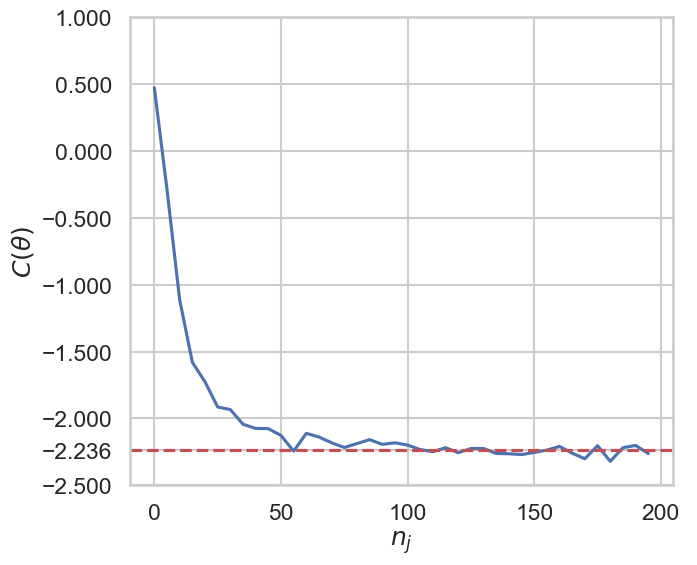
\includegraphics[width=\textwidth]{vqe-result-1.png}
            \caption{Graph of Cost function vs Iterations}
            \label{fig:vqe-results-1}
        \end{subfigure}
        \hfill
        \begin{subfigure}[t]{0.5\textwidth}
            \centering
            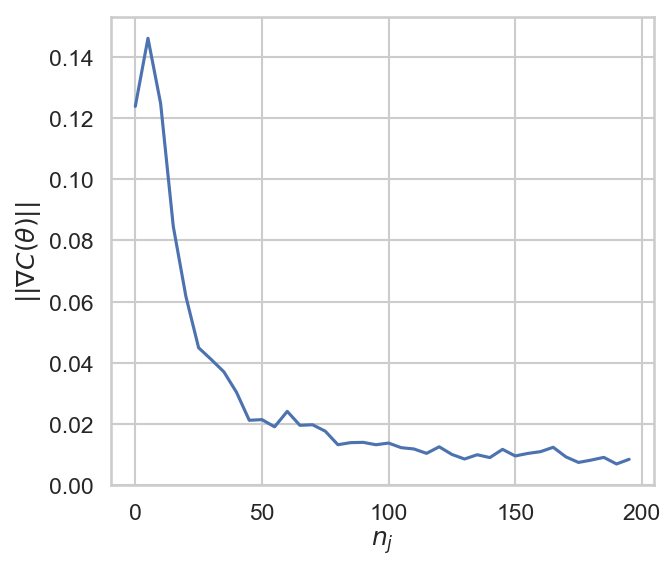
\includegraphics[width=\textwidth]{vqe-result-2.png}
            \caption{Graph of Gradient norm vs Iterations}
            \label{fig:vqe-results-2}
        \end{subfigure}
    }
    \caption{Results of VQE for the setup described}
    \label{fig:vqe-results}
\end{figure}

Graph of cost function $C(\boldsymbol{\theta})$ is plotted against number of iterations of the hybrid quantum-classical loop in \ref{fig:vqe-results-1}. As is expected from the simple nature of the problem and small parameter set, the cost function decreases sharply within the first few iterations, similar to exponential decay. This corresponds to "larger" steps across the cost landscape, as is evident from the large values of gradient norm shown in fig \ref{fig:vqe-results-2}, which also fall exponentially. 

The large drop in cost upto $n_j = 50$ corresponds to the optimizer descending in direction of the largest gradients (in terms of gradient norm), and the circuit learns a value close to the expected theoretical minimum (shown by a dashed red line in \ref{fig:vqe-results-1}). Hence, we conclude that the ansatz even at $d = 4$ is expressive enough for the problem. In the iterations following that we see convergence to the minimum with minor fluctuations. Since, this is being executed on a local simulator, this cannot be attributed to hardware noise, rather, this can be explained due to stochastic and simplistic nature of the gradient descent optimizer which may cause it to overshoot beyond the global minima on the cost landscape. Further, we can state that due to low depth the circuit is not able to increase convergence quickly, whereas with higher depth stronger convergence could be achieved. The infidelity obtained was $\sim 10^{-4}$ indicating very strong convergence of the circuit parameters to the actual ground state. Overall, this could be interpreted as evidence of the success of VQAs at solving basic domain-specific problems using shallow depth and low qubit count devices.

Suggested methods for further research would be to simulate hardware noise as well, to determine how well the algorithm runs on modern day hardware.

\textbf{Varying hyperparameters:} We search through the space of different hyperparameters, to find the set such that:
\begin{itemize}
    \item Cost function converges the fastest
    \item Solver provides consistent values
    \item Balances expressivity and accuracy with computational cost
\end{itemize}

To compare the results, we calculate the theoretical minimum using an exact eigensolver, and evaluate infidelity of the final state obtained. The same setup as above is reused with only the hyperparameter in study being varied.

\begin{figure}[H]
    \centering
    \makebox[\textwidth]{
        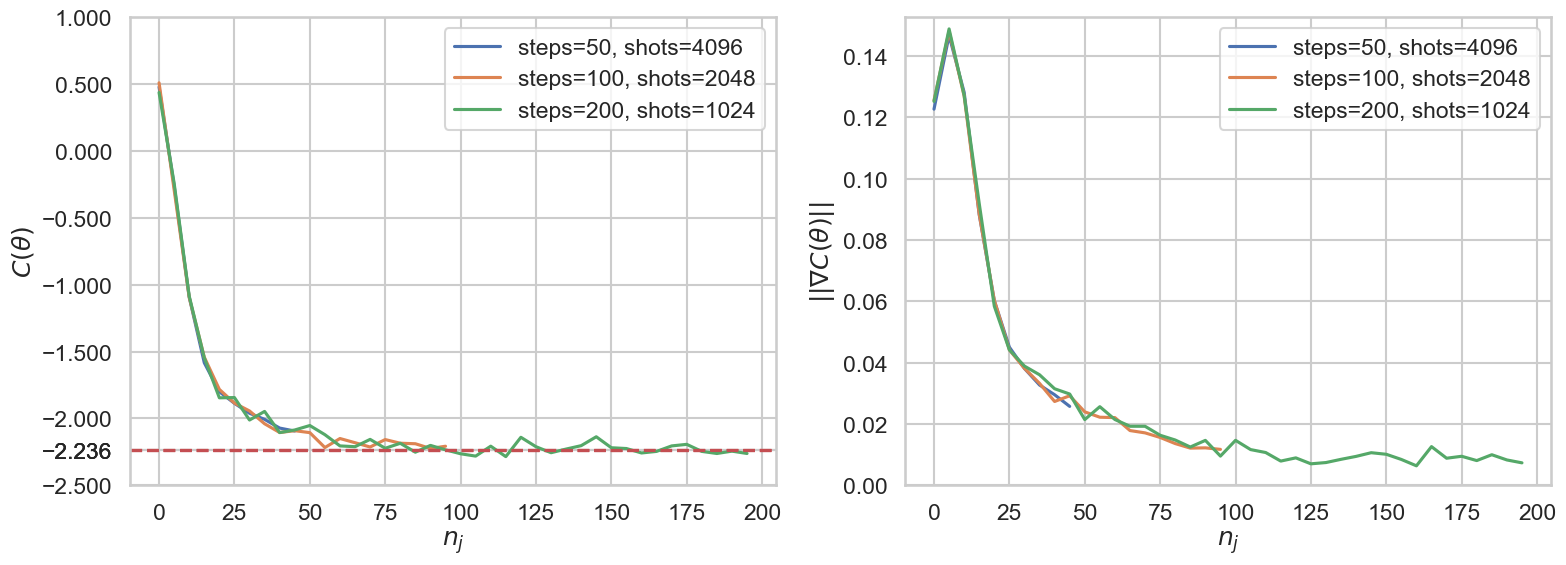
\includegraphics[width=1.1\textwidth]{vqe-vary-1.png}
    }
    \small
    \begin{tabular}{@{}llll@{}}
        \toprule
        \textbf{Model No.}  & \textbf{Steps} & \textbf{Shots} & \textbf{Infidelity} \\ \midrule
        1. & 50  & 4096 & $8 \cdot 10^{-2}$ \\
        2. & 100 & 2048 & $1 \cdot 10^{-2}$ \\
        3. & 200 & 1024 & $2 \cdot 10^{-4}$ \\ \bottomrule
    \end{tabular}
    \caption{Results and performance metrics of varying the steps or number of iterations with the number of shots of the VQE}
    \label{fig:vqe-vary-1}
\end{figure}

Fig. \ref{fig:vqe-vary-1} shows the variation of the steps or number of iterations $N$, and the number of shots used by the \texttt{EstimatorV2} object in Qiskit, which is equivalent to the accuracy of estimation, while keeping total computational cost fairly constant. Higher number of shots lead to better estimation of gradient at the cost of lesser optimization loop iterations. We find that $N = 200$ and $\text{shots} = 1024$ gives better accuracy and lower spread, with least infidelity though it takes longer to converge.

\begin{figure}[H]
    \centering
    \makebox[\textwidth]{
        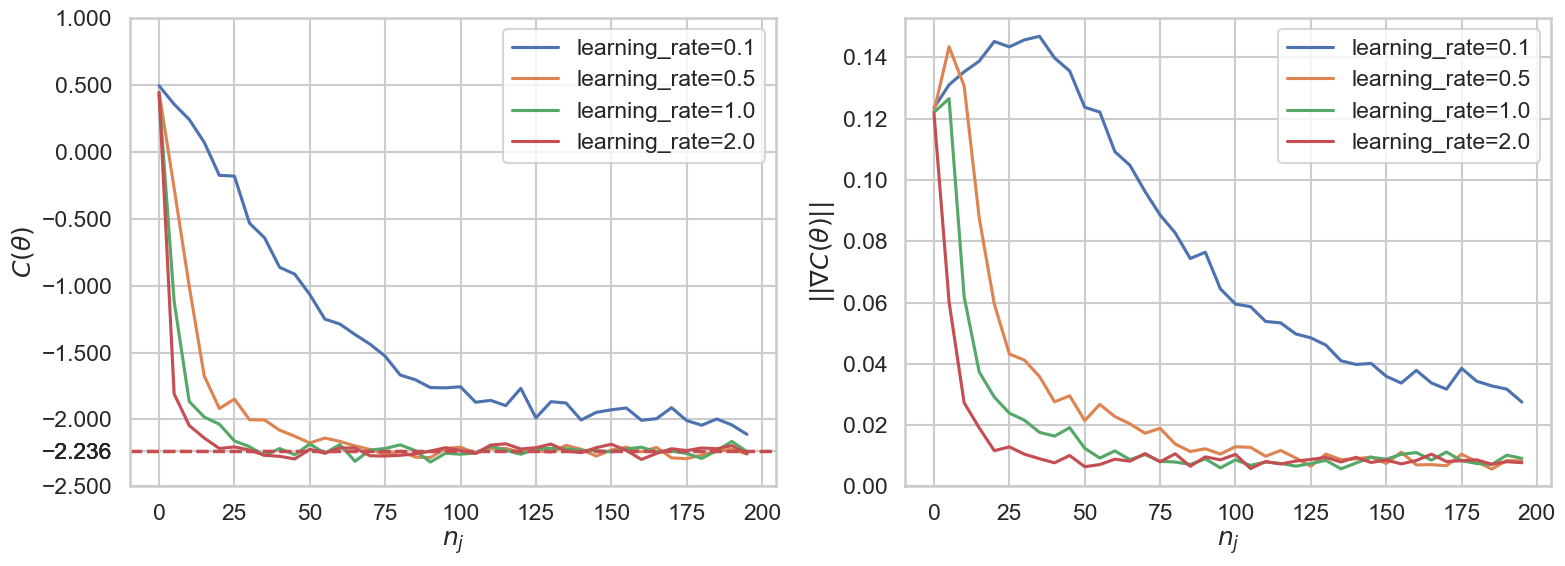
\includegraphics[width=1.1\textwidth]{vqe-vary-2.png}
    }
    \small
    \begin{tabular}{@{}lll@{}}
        \toprule
        \textbf{Model No.}  & \textbf{Learning rate} & \textbf{Infidelity} \\ \midrule
        1. & 0.1 & $1 \cdot 10^{-1}$ \\
        2. & 0.5 & $1 \cdot 10^{-3}$ \\
        3. & 1.0 & $5 \cdot 10^{-5}$ \\
        4. & 2.0 & $9 \cdot 10^{-5}$ \\ \bottomrule
    \end{tabular}
    \caption{Results and performance metrics of varying the learning rate of the SGD optimizer}
    \label{fig:vqe-vary-2}
\end{figure}

Fig. \ref{fig:vqe-vary-2} shows the variation of the learning rate ($\eta$) over the space $[0.1, 0.5, 1, 2]$. Lower values of $\eta$ can cause slow convergence but we may get stuck in suboptimal minimas.  Higher $\eta$ can lead to faster convergence but we also skip over sharp, optimal minimas and cause divergence, reducing consistency. We find that $\eta = 1$, gives the fastest convergence and drastically lower infidelity. It avoids the larger fluctuations associated with $\eta = 2$.  

\begin{figure}[H]
    \centering
    \makebox[\textwidth]{
        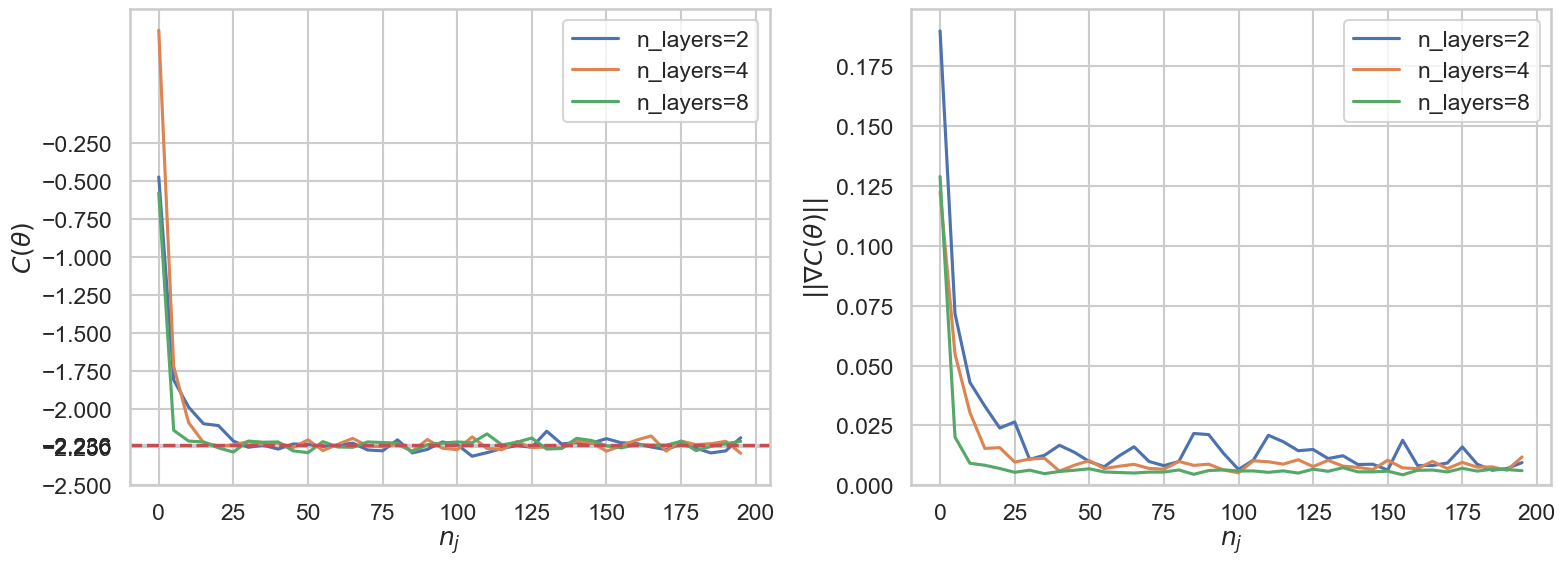
\includegraphics[width=1.1\textwidth]{vqe-vary-3.png}
    }
    \small
    \begin{tabular}{@{}lll@{}}
        \toprule
        \textbf{Model No.}  & \textbf{Depth} & \textbf{Infidelity} \\ \midrule
        1. & 2  & $2 \cdot 10^{-3}$ \\
        2. & 4  & $7 \cdot 10^{-5}$ \\
        3. & 8  & $5 \cdot 10^{-5}$ \\ \bottomrule
    \end{tabular}
    \caption{Results and performance metrics of varying the number of layers of the hardware efficient ansatz (HEA)}
    \label{fig:vqe-vary-3}
\end{figure}

Finally, fig. \ref{fig:vqe-vary-3} shows the variation of the number of layers ($d$ represented by \textit{n\_layers} in the plot) of the ansatz over the space $[2, 4, 8]$. Lower values allows for easier trainability but risks losing expressibility. Higher values increases expressibility but makes the optimization harder and introduces the problem of barren plateaus. We find that $d = 2$ exhibits lower expressibility than the other two choices, which can be observed in terms of the larger gradient norms. Clearly, $d = 8$ provides the best results in terms of fidelity as less convergence of cost function. Nonetheless, $d = 4$ is also sufficiently expressible to learn the ground state accurately, along with drastically lower computation cost due to fewer parameters.

\subsection{Summary}

We have applied the concepts of variational quantum algorithms to a quantum circuit of shallow depth and low qubit count, in order to train variational parameters thereof, which was used to estimate the ground state and ground energy of a Hamiltonian based on the variational principle. Along with learning cutting-edge quantum computing techniques, we have developed a method to map simple variational problems onto quantum circuits which can be optimized by ML-inspired methods.

We observe that using even a circuit of depth $d=4$ with $n = 2$ qubits, is sufficient to solve a problem of this scale, which is promising for real quantum hardware execution. We have also analyzed and interpreted the effect of varying the hyperparameters associated with this model. For improving accuracy, one can consider increasing the depth of the circuit to increase expressiblity, while making sure that the parameters are correctly initialized to prevent vanishing gradients, and prevent the problem of barren plateaus. Finally, the learning rate is an important parameter that must be chosen carefully to ensure fastest convergence while preventing too large jumps in the cost landscape.

Suggested methods for future research include using sophisticated optimizers such as Adam, AdaGrad. More complex hamiltonians can be used to capture more complicated systems, which allows exploring more complex ansatz topologies with richer entangling behaviours.

\section{DQCs and a nonlinear differential equation solver} \label{sec:DQC}

\subsection{Introduction}

Differential equations (DEs) are central to modeling a wide variety of physical, biological, and economic systems, but, solving them analytically becomes challenging as systems grow in complexity. Classical solvers typically rely on discretization techniques, such as finite difference methods, or global approaches, like spectral methods, both of which are computationally expensive for high-dimensional or nonlinear systems. Using quantum computing, we explore a fundamentally new approach by leveraging quantum states to represent complex solutions compactly.

Quantum methods offer speedup in specific cases due to the exponential scalability of quantum state representations. Algorithms like the HHL algorithm for linear systems are promising for solving linear DEs by encoding solutions in amplitude space, although they face challenges such as data input and readout problems. Hence, we introduce differentiable quantum circuits (DQCs) which extend these ideas to nonlinear DEs. The key benefits of this method are that it involves embedding functions into quantum feature maps which allow for easier search for global solutions, and it uses automatic differentiation to calculate derivatives directly, bypassing the numerical inaccuracies of classical finite difference methods.

\subsection{Basic Tools and Worflow}

\begin{figure}[H]
    \centering
    \makebox[\textwidth]{
        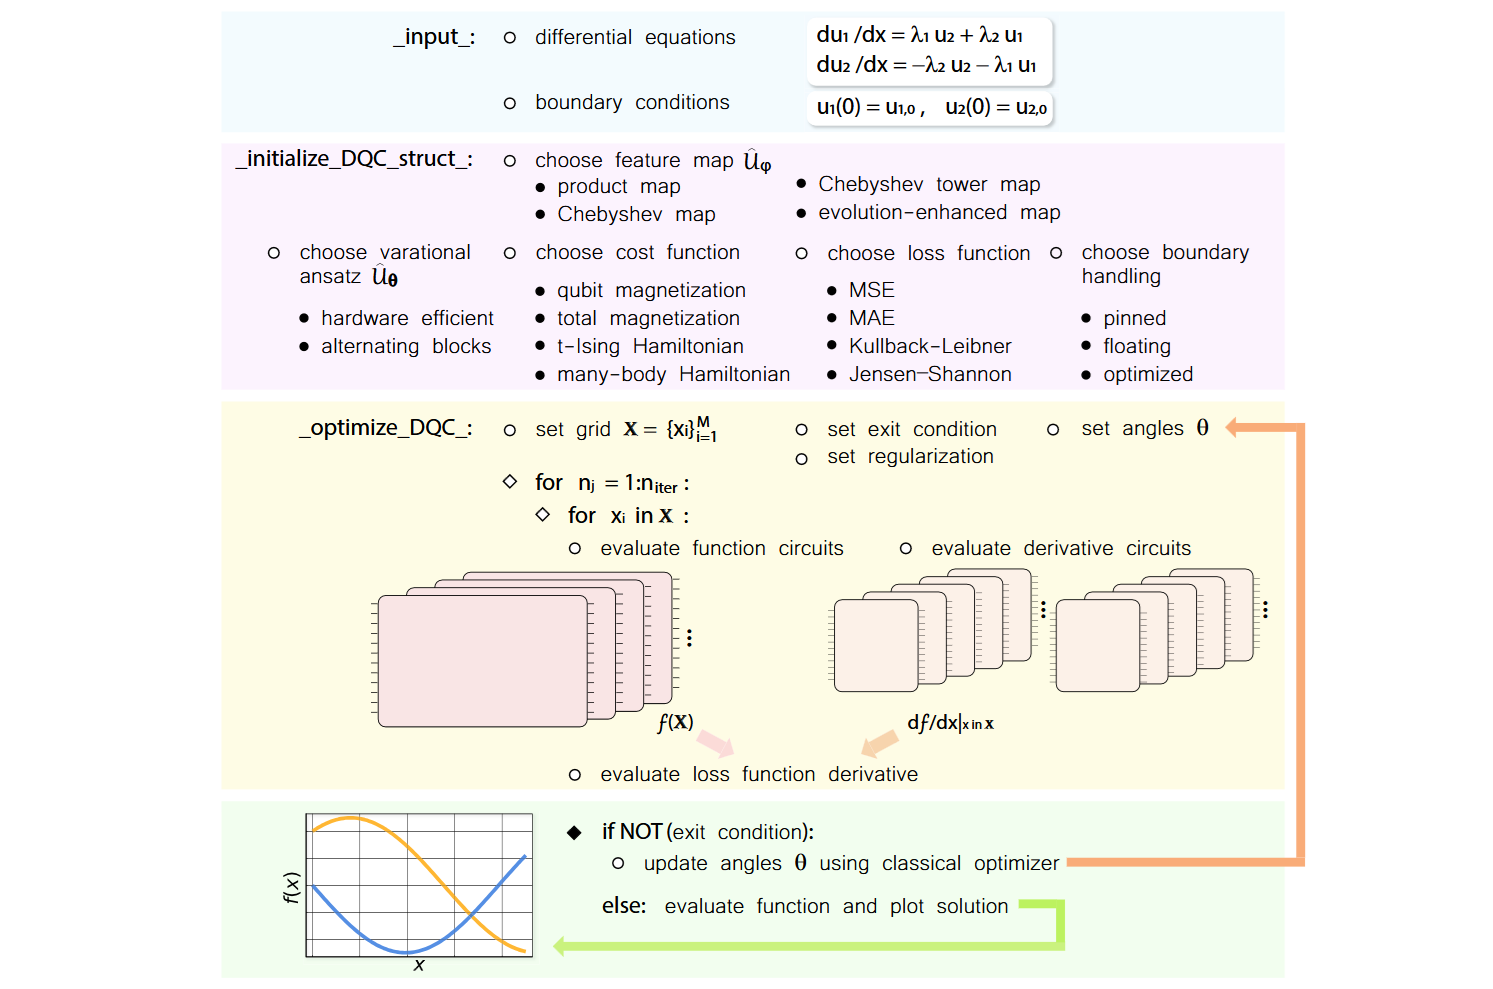
\includegraphics[width=1.25\textwidth]{dqc-optimization-workflow.png}
    }
    \caption{\textbf{DQC Optimization Workflow}: Adapted from \cite{DQC}.}
    \label{fig:dqc-optimization-workflow}
\end{figure}

This section provides an overview description of differential equation (DE) solver. The trial solutions of the DE system are prepared as quantum circuits parameterized by the independent variable(s) $x \in \mathbb{R}^{\nu}$ (collection of $\nu$ variables in general). This involves applying a quantum feature map $\hat{\mathcal{U}}_\varphi(x)$ to encode the predefined nonlinear function $\varphi(x)$ as amplitudes of the quantum state. Unlike amplitude encoding used in the HHL algorithm, feature map does not require access to all amplitudes individually; it is a latent space representation of the multi-qubit state. Next, we add a variational quantum circuit $\hat{\mathcal{U}}_\theta(x)$ parametrized by $\boldsymbol{\theta}$ which is optimized in a quantum-classical optimization loop. The real valued trial function is estimated as an expectation value of a predefined Hermitian cost operator $\hat{\mathcal{C}}$ as $f(x) = \bra{f_{\varphi,\theta}(x)}\hat{\mathcal{C}}\ket{f_{\varphi,\theta}(x)}$, where $\ket{f_{\varphi,\theta}(x)} = \hat{\mathcal{U}}_\theta\hat{\mathcal{U}}_\varphi(x) \ket{\O}$. Evaluation of the derivative function is done by differentiating the quantum feature map circuit using the product rule and chain rule, with a technique known as automatic differentiation (AD), which allows the function derivative to be represented by its exact analytic formula as opposed to numerical methods. Finally, we define the optimization goal using the loss function $\mathcal{L}_\theta[d_x f, f, x]$ which consists of error terms with respect to the trial function, boundary condition and optionally, a set of regularization points. This is used to solve the optimization problem $\boldsymbol{\theta}_\text{opt} = \arg\min_\theta \mathcal{L}_\theta[d_x f, f, x]$ at the set of points $\mathbb{X} = \{x_i\}_{i=1}^M$.

\subsubsection{Quantum feature maps}

A quantum feature map effectively maps the computational state space onto a latent space spanned by a rich basis of non linear functions that can approximate the solution function to a high degree. Some useful maps are explored here.

\textbf{Product feature maps.} This map involves layers of single qubit rotations with a non-linear dependence $\varphi[x]$ of encoded in $x$. In the single layer case it can wrriten as

$$\mathcal{\hat{U}}_\varphi(x) = \bigotimes_{j=1}^{N'} \hat{R}_{\alpha,j}(\varphi[x])$$

where $N' \leq N$ is the number of qubits used for encoding, $\alpha$ refers to the rotation axis and $j$, the qubit to operate on.

$\alpha = y, \varphi(x) = \arcsin x$ is a well-known choice.

The derivative for a unitary operator in the form of an involutory matrix (as is the case of length-1 Pauli string here) can be simplified using the standard parameter shift rule as:

$$
\frac{d}{dx} \langle \O | \mathcal{\hat{U}}_\varphi(x)^\dagger \hat{C} \mathcal{\hat{U}}_\varphi(x) | \O \rangle
= \frac{1}{4} \left( \frac{d}{dx} \varphi(x) \right) \big( \hat{\braket{C}}^+ - \hat{\braket{C}}^- \big)
$$

where $\hat{\braket{C}}^\pm$ are the sums of the shifted unitaries computed as per the parameter shift rule, with a shift of $\frac{\pi}{2}$.

\textbf{Chebyshev feature maps}. It is the map with the choice of $\varphi(x) = 2n \arccos x$ ($n$ varies with $j$) and $\alpha = y$ for real amplitudes . This has the effect of a unitary operation with matrix elements defined by $n$-degree Chebyshev polynomials of first and second kind ($T_n(x), U_n(x)$ respectively). The power of this representation can be inferred from approximation theory which states that any smooth function can be represented as $f(x) = \sum_{n=0}^{\infty} A_n T_n(x), \quad |x| \leq 1$.

This has two variants, the first being \textit{sparse Chebyshev feature map} with $n=1$, ensuring that the encoded degree is homogenous and equal to one, allowing for a simple representation. Due to the nonlinearity introduced by Chebyshev polynomial, this mapping is very effective for mapping oscillatory features.

The basis set can be further enriched by considering the \textit{Chebyshev tower feature map}, where $n$ varies as $n[j] = j$, increasing the expressibility without increasing the number of rotations.

\textbf{Evolution enhanced feature maps.} The above maps produce states that are limited to the product state space. To span the entire Hilbert space we need to populate the entangled substates which can be done by means of a time evolution corresponding to a complex Hamiltonian $\hat{H}$ over a time $\tau$ (may be constant or varied variationally or non-variationally).

\subsubsection{Variational quantum circuit}

In this section we primarily discuss the case of hardware efficient ansatz in particular, as a general discussion has been included in sec. \ref{sec:Ansatz}. The structure used here consists of $\hat{R}_z - \hat{R}_x - \hat{R}_z$ (or similar) rotation gates parametrized independently, followed a global entangling layer made using \texttt{CNOT} gates. The expressivity grows with depth $d$.

Alternating blocks ansatz is a good alternative where instead of global entangling layers, seperate sublocks are used, which are shifted and repeated in a checkerboard like manner. The idea is to introduce local entanglement behaviour which gradually forms a globally correlated state, however this is may lead to problems in trainability especially if random initalization is used.

\subsubsection{Cost function}

A Hermitian cost operator $\mathcal{\hat{C}}$ is used to measure the trial function $f(x)$ as an observable. The simplest choice is magnetization of a single qubit $j$, $\braket{\hat{Z}_j}$. This allows representing functions in range $[-1, 1]$. Similarly, total magnetization or $\mathcal{\hat{C}} = \sum_j \hat{Z}_j$ is a good choice, where the weights can be varied. This is suitable due to efficient hardware implementation and the symmetrical nature of the operator.

More complex alternatives are T-Ising Hamiltonian which includes nearest-neighbour spin coupling ($\braket{\hat{Z}_j \hat{Z}_{j+1}$) and external magnetization field terms ($\braket{\hat{X}_j}$) along with individual spin terms ($\hat{Z}_j$). One can also use a set of Pauli strings as was done in the VQE example discussed before, inspired from quantum chemistry. Finally, a linear combinations of different cost functions can be used $\mathcal{\hat{C}} = \sum_\ell \alpha_\ell \mathcal{\hat{C}}_\ell$, with the coefficients being optimized at par with the variational parameters of the ansatz.

\subsubsection{Loss function}

Finally, the loss function provides a way to quantify how well the predicted trial function matches the required conditions. It can be expressed as a sum of contributions from how well the differentials match the functional, with the accuracy of the boundary conditions, as well as (optionally) the distance from a set of regularization points.

$$
\mathcal{L}_{\boldsymbol{\theta}} [d_x f, f, x] = \mathcal{L}^{\text{(diff)}}_{\boldsymbol{\theta}} [d_x f, f, x] + \mathcal{L}^{\text{(boundary)}}_{\boldsymbol{\theta}} [f, x] + \mathcal{L}^{\text{(reg)}}_{\boldsymbol{\theta}} [f, x]
$$

The differential loss is defined as mean loss of the functional $F[d_x f, f, x]$ over the training grid $\mathbb{X}$. Different loss types are considered, with the simplest choice being \textit{mean square error} (MSE), followed by \textit{mean absolute error} (MAE), or more complex versions like Kullback-Liebler divergence and Jensen-Shannon divergence.

\subsubsection{Boundary handling}

Along with approximating the functional to a high degree of accuracy, it is important that the solver handles the initial value or boundary value problem effectively. This can be handled via these 3 methods:

\textbf{Pinned boundary handling}. This involves including the information about the boundary in the expectation of the cost function itself. The boundary term in the loss function encodes this using a simple loss type such as MSE, scaled by a constant.

$$
\mathcal{L}^{\text{(boundary)}}_{\boldsymbol{\theta}} [d_x f, f, x] = \eta \left( f_{\boldsymbol{\theta}}(x_0) - u_0 \right)^2
$$

This allows equivalent treatment of boundary and derivative terms. The weakness is that it requires a constant times identity term ($\alpha_0\mathbb{I}$) be added to the cost operator such that the expectation at $\boldsymbol{\theta}_\text{init}$ lies close to $u_0$ at $x = x_0$.

\textbf{Floating boundary handling}. Here, the estimated solution is corrected by iteratively computing a constant to shift the expectation value by, in order to match the boundary condition, that is

\begin{align*}
f(x) = f_b + \bra{f_{\varphi, \boldsymbol{\theta}}(x)} \mathcal{\hat{C}} \ket{f_{\varphi, \boldsymbol{\theta}}(x)}
\\
f_b = u_0 - \bra{f_{\varphi, \boldsymbol{\theta}}(x_0)} \mathcal{\hat{C}} \ket{f_{\varphi, \boldsymbol{\theta}}(x_0)}
\end{align*}

This neither requires a seperate loss term, nor it be encoded in the cost operator. It guarantees exact matching, but requires knowledge of the exact initial value which may be a problem in some cases. In cases where the expectation at $x = x_0$ lies far from $u_0$, this can lead to issues in training due to large variations in $f_b$.

\textbf{Optimized boundary handling}. Similar to floating boundary handling, it proposes adding a constant to the expectation value but it is optimized using gradient descent, similar to the variational parameters. This removes the need to include boundary information in the cost operator, but it must be included in the loss function. This helps in quickly rectifying the parameter when the boundary condition is heavily mismatched, however the combined terms in the loss function may compete during optimization.

\subsubsection{Regularization}

Regularization is a technique to guide the optimizer towards the true solution, that is, the global minima, by feeding in prior information about the potential solution. This involves defining a set of regularization points $\{ x_\text{reg} \}_{r=1}^R$ with corresponding function values $\{ u_\text{reg} \}_{r=1}^R$. An additional loss term is then defined, using, say, MSE loss, whose contribution can be scaled according to an optimization schedule. In general, we require higher emphasis on the regularization-based training during initial iterations, which should diminish to zero at later stages (for e.g., to prevent overfitting). Linearly decreasing or reverse sigmoid based optimization schedules are considered.

\subsection{Methodology - Examples}

In this section, we discuss application of the above worflow to two basic examples of ordinary differential equations (ODEs) using a subset of the methods discussed here.

We build the DQC-based solver using the Qadence Python library to implement the circuit because of its expressive workflow for training quantum machine learning models. The \texttt{QNN} class is used to instantiate the model. It is executed on the default PyQTorch backend with automatic differentiation enabled using the \texttt{autograd} engine from PyTorch. It is built on a full quantum state simulator in a noiseless setting.

The HEA ansatz structure is used with $\hat{R}_z-\hat{R}_x-\hat{R}_z$ rotation gates as obtained from the \texttt{hea} method provided by Qadence. We explore variations of the feature map and ansatz hyperparameters to find their effect on solution convergence. In this setup, we use \textit{pinned boundary handling}.

\subsubsection{Example 1}
We choose the single ODE that is

\begin{equation} \label{eq:first}
    \frac{du}{dx} + \lambda u (\kappa + \tan(\lambda x)) = 0, \quad u(0) = u_0
\end{equation}

Whose analytic solution is known in the form of a damped oscillating function

$$
u(x) = u_0 e^{-\kappa\lambda x} \cos(\lambda x)
$$

While the problem is fairly simple being a single ODE, it captures both oscillatoric and decaying features which requires a rich basis set of functions for close fitting.

We take the case of $\lambda = 8$, for $\kappa = 0.1, u_0 = 1$. Optimization grid is taken as a set of 20 equidistant points from $x = 0$ to $x = 0.9$, due to diverging derivatives of the $\arccos$ function used in feature map, at $x = 1$. A quantum register with $N = 6$ qubits is chosen, on hardware-efficient ansatz with $d = 6$. Total magnetization cost function is used to read out the trial function, due to its efficient implementation. MSE loss function is used wherever applicable.
\\\\
\textbf{Pinned boundary handling}\\
Pinned boundary handling has been used in this case, with a boundary loss weight coefficient, optimized on a per-case basis, to balance the differential and boundary loss terms for smoother optimization. It is chosen as $50.0$ in case of Chebyshev (sparse) map, and $0.001$ in the case of Chebyshev tower map. This can be explained by the difference in expressibilities of the two feature map, as the more expressive basis set provided by Chebyshev tower map  can adequately minimize the boundary loss term along with the differential residual, whereas the Chebyshev (sparse) map requires "higher emphasis" on the boundary loss term.

As described in the 'pinned boundary handling' method above, a constant times identity term is added to the cost observable. Here, we use a constant simply determined as $\alpha = u_0 - f_{\varphi, \boldsymbol{\theta_\text{init}}}(x_0)$. This ensures that the overall circuit unitary has produces result close to $u_0$ at $x = x_0$ at $\boldsymbol{\theta_\text{init}}$.
\\
The training regime consists of $1200$ epochs trained using Adam with a learning rate of $0.01$.

\subsubsection{Example 2}
We choose the single ODE that is

\begin{equation} \label{eq:second}
    \frac{du}{dx} - 4u + 6u^2 - \sin(50x) - u\cos(25x) + \frac{1}{2} = 0, \quad u(0) = u_0
\end{equation}

The solution is hard to represent analytically and has various high frequency oscillatoric and non-oscillatoric terms representing growth and decay, which will better highlight the power of rich feature maps in solving differential equations.
The problem is setup with $u_0 = 0.75$ with training grid taken as a set of 100 equidistant points from $x = 0$ to $x = 0.9$ (same as example 1). Same as above, we use pinned boundary handling with the weights optimized seperately.
\\\\
\textbf{Method 1}\\
First, we explore different ansatzes of varying depth $d = 6, 12$ to study how the convergence rate and final solution accuracy is affected by depth. A quantum register with $N = 8$ qubits is chosen to provide a larger set of Chebyshev basis functions with higher degree polynomials which are needed in this case. Adam optimizer is used to train over 1000 epochs. The increase in parameters due to 8 qubits, leads to a more complex loss landscape and larger capacity of the model, so we use a smaller learning rate of 0.001 in this case. Boundary loss weight $10.0$ is used in both cases.
\\\\
\textbf{Method 2}\\ 
We use both the standard Chebyshev tower feature map, as well as the evolution enhanced (EvEn) feature map to study the increase in expressibility offered by the latter which is will be useful in approximating more complex functions. Here, hyperparameters $N=6$ and $d=6$ are used. The model is first trained over 500 epochs using Adam with the \texttt{ChebT} feature map, and parameters thus obtained are passed on to an updated unitary with the \texttt{EvEn} feature map which is further trained over 500 epochs. Learning rate of 0.01 is used, with boundary loss weight $50.0$.

\begin{figure}[H]
    \centering
    \makebox[\textwidth]{
        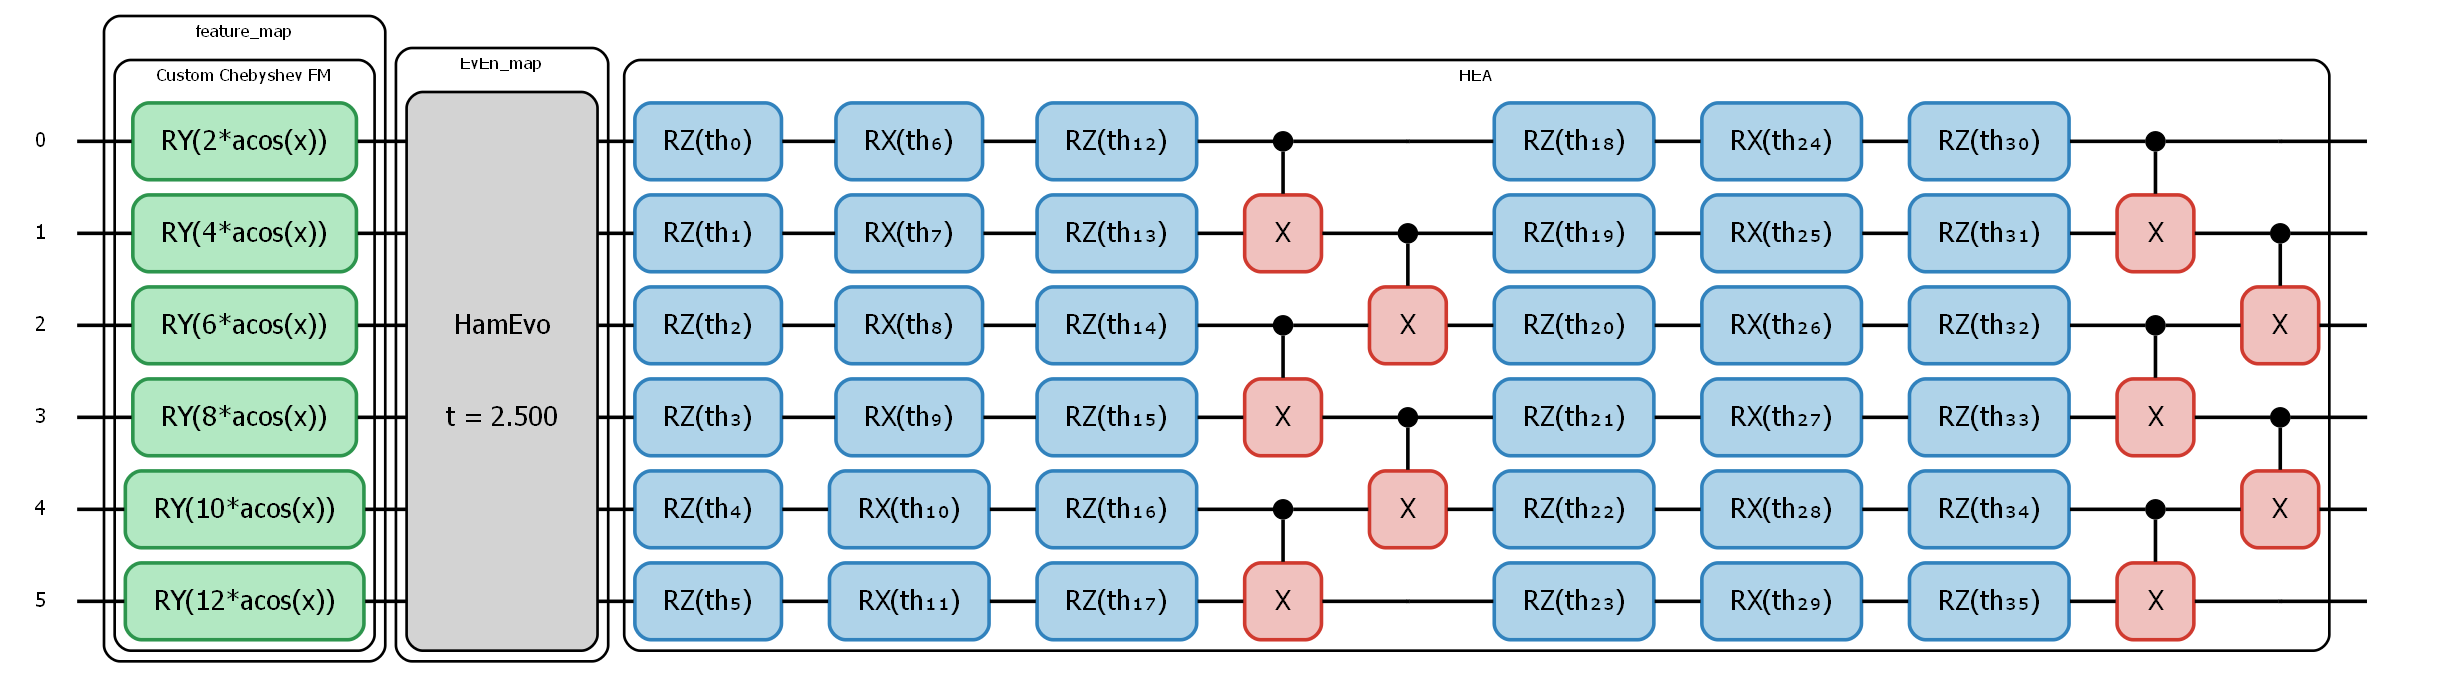
\includegraphics[width=1.2\textwidth]{EvEn-circuit.png}
    }
    \centering
    \caption{\textbf{Illustration of EvEn feature map circuit created using Qadence} only 2 out of 6 HEA layers are shown for clarity}
    \label{fig:EvEn-circuit}
\end{figure}

For the time evolution, we make use of a T-Ising model Hamiltonian defined as $\hat{H} = \sum_{i} J_{j,j+1}\hat{Z}_{j}\hat{Z}_{j+1} + h^{z}_{j} \hat{Z}_j + h^{x}_{j} \hat{X}_j$ with the weights being randomly assigned from $[-1, 1]$. A constant evolution time of $\tau = 2.5$ is used for applying the unitary evolution $\exp{(-i\hat{H}\tau)}$.

\subsection{Results and Interpretation}

To solve the first equation, we explore the \textit{Chebyshev (sparse) feature map} and the \textit{Chebyshev tower feature map}. To measure performance of the model we plot the total loss function $L_F$ as well as the "quality of solution" obtained $L_Q$, that is, the MSE loss between the model's predicted function with the true solution over the set of testing grid points. Logarithmic scale is used on the y-axis.
\begin{figure}[H]
    \centering
    \makebox[\textwidth]{
        \begin{subfigure}[t]{0.45\textwidth}
            \centering
            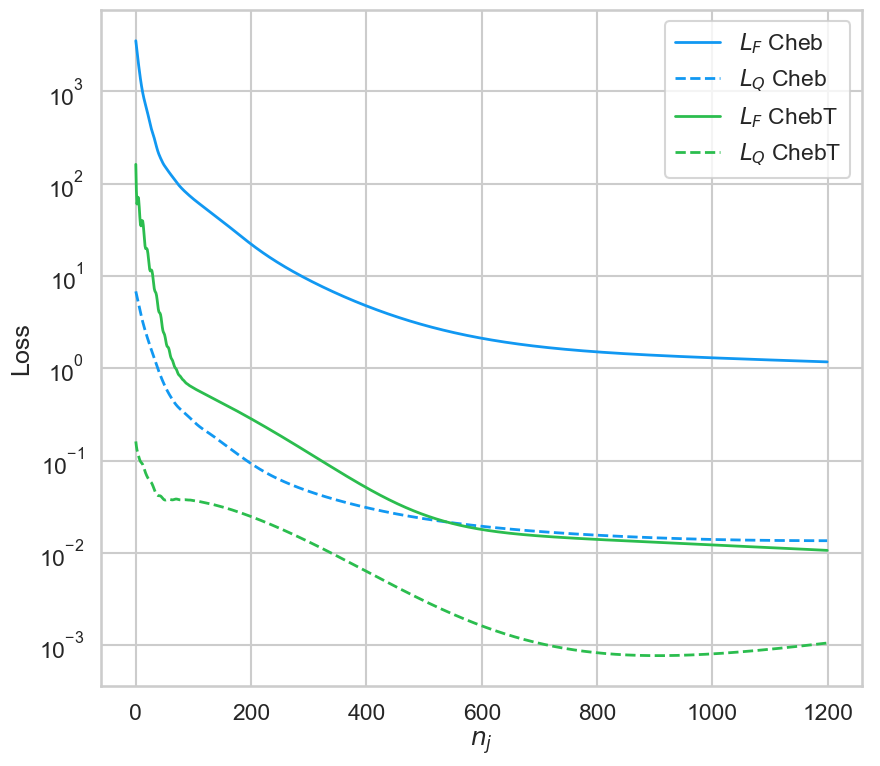
\includegraphics[width=\textwidth]{dqc-results-1-1.png}
            \caption{\textbf{Graph of Loss function over Iterations} \\
            Full loss $L_F$ is shown as solid lines, quality $L_Q$ as dashed lines. }
            \label{fig:dqc-results-1-1}
        \end{subfigure}
        \hfill
        \begin{subfigure}[t]{0.45\textwidth}
            \centering
            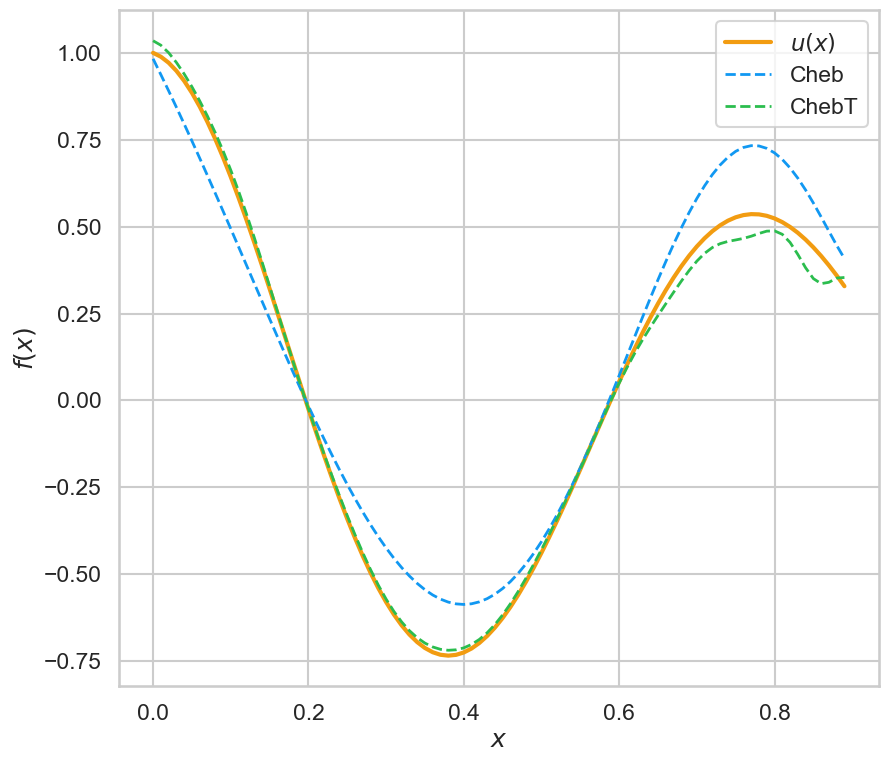
\includegraphics[width=\textwidth]{dqc-results-1-2.png}
            \caption{\textbf{Graph of corresponding trained solutions alongside known solution (shown as solid line)}}
            \label{fig:dqc-results-1-2}
        \end{subfigure}
    }
    \caption{\textbf{Results of DQC solver implemented for eq. \ref{eq:first}}}
    \label{fig:dqc-results-1}
\end{figure}

Fig. \ref{fig:dqc-results-1-1} shows the total loss function $L_F$ as a function of number of iterations as solid lines. We notice a steep descent in first 100 iterations corresponding to larger steps across the cost landscape, with minor oscillations due to the stochastic nature of the optimizing strategy and because of the model adjusting to boundary conditions. Further, the loss function decrease rate slows and stabilizes corresponding to an approximate solution being found which is being further optimized. Finally, loss plateaus around $10^0$ in the case of Chebyshev map (shown in blue) and around $10^{-2}$ in the case of Chebyshev tower map (shown in orange).

We observe that the Chebyshev tower map converges closer to the true solution ($L_Q$ plateaus around $10^{-3}$) due to the richer basis set of functions at $N = 6$ qubits, and, it is able to better learn the oscillatoric features of the equation.

It is clear that the Chebyshev (sparse) map takes longer to converge. Still it is able to broadly learn the oscillatoric as well as decaying features ($L_Q$ plateaus around $10^{-2}$).

\\ \\\\

To solve eqn. \ref{eq:second}, we explore the \textit{Chebyshev tower feature map} with differing ansatz depths, and an evolution enhanced (EvEn) feature map.

\begin{figure}[H]
    \centering
    \makebox[\textwidth]{
        \begin{subfigure}[t]{0.45\textwidth}
            \centering
            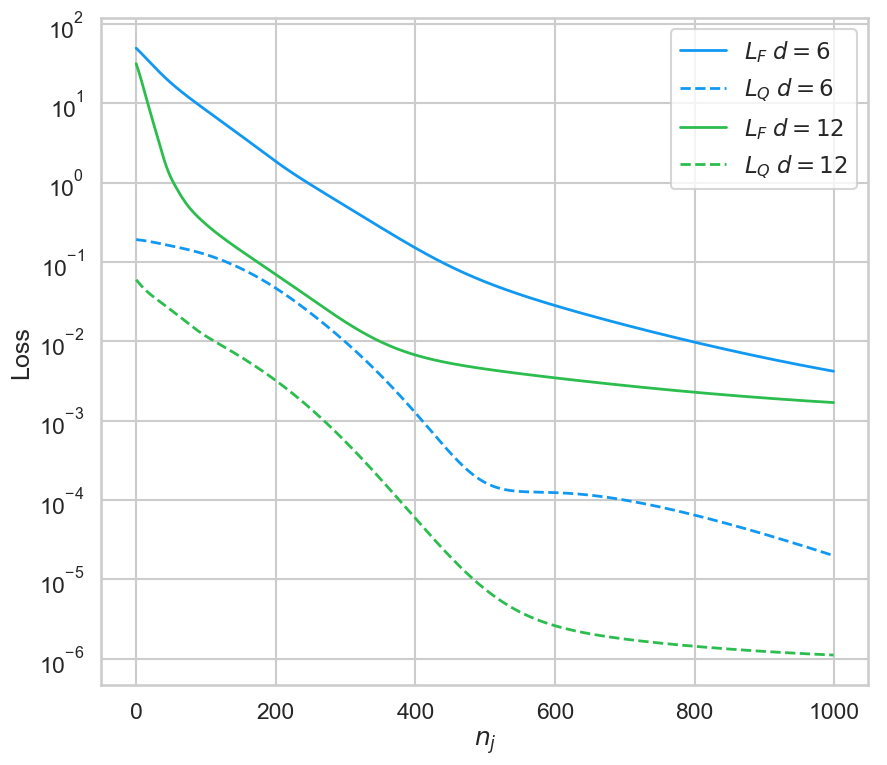
\includegraphics[width=\textwidth]{dqc-results-2-1.png}
            \caption{\textbf{Graph of Loss function over Iterations}\\
            Full loss $L_F$ is shown as solid lines, quality $L_Q$ as dashed lines.}
            \label{fig:dqc-results-2-1}
        \end{subfigure}
        \hfill
        \begin{subfigure}[t]{0.45\textwidth}
            \centering
            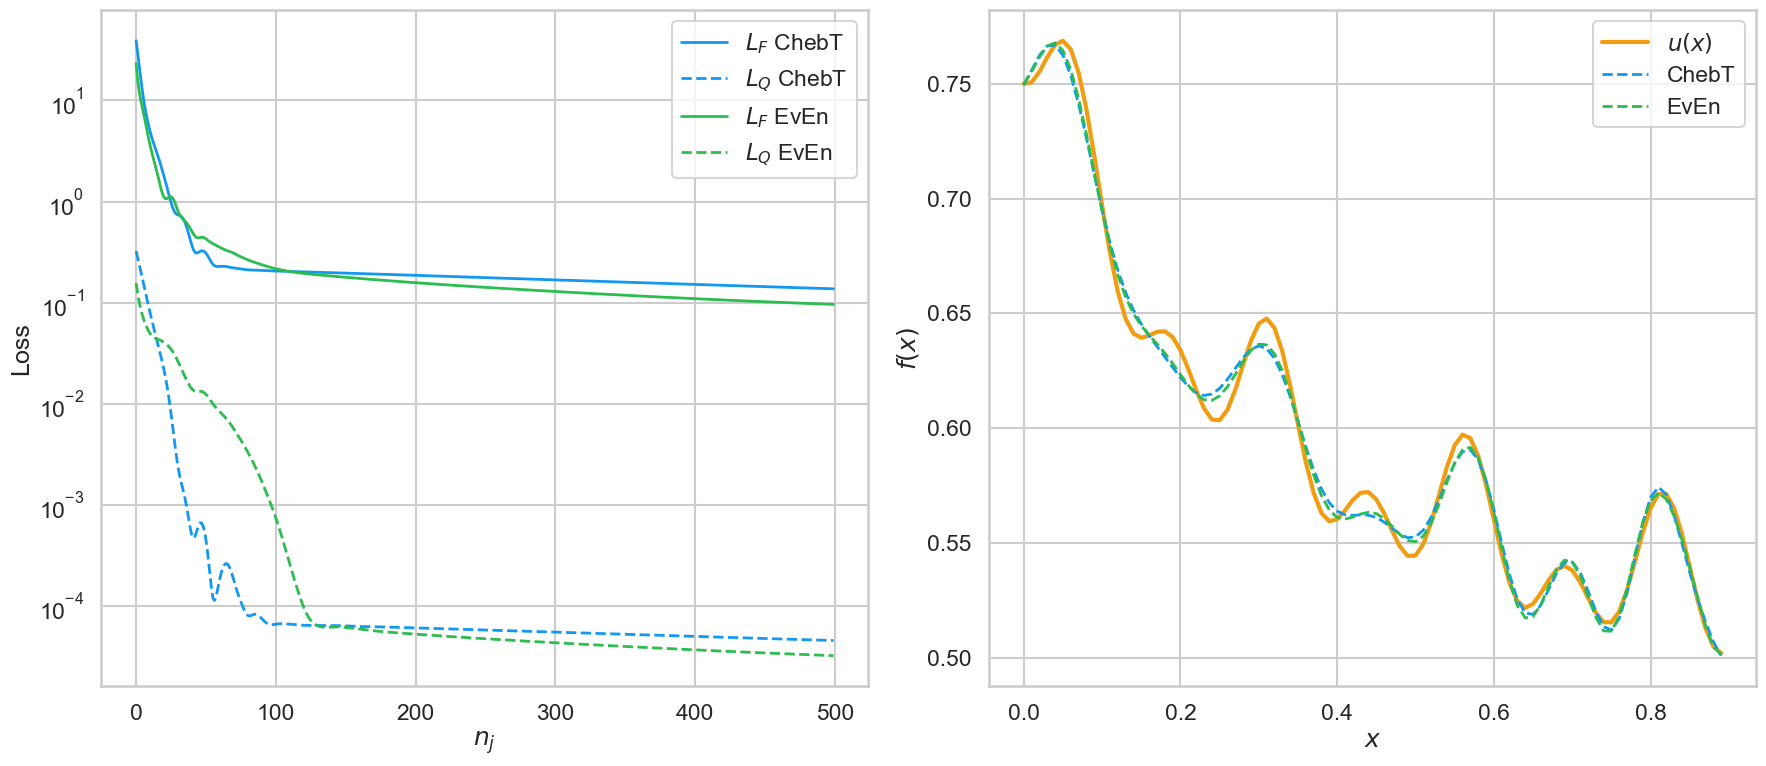
\includegraphics[width=\textwidth]{dqc-results-2-2.png}
            \caption{\textbf{Graph of corresponding trained solutions alongside known solution (shown as solid line)}}
            \label{fig:dqc-results-2-2}
        \end{subfigure}
    }
    \caption{\textbf{Results of DQC solver implemented for eq. \ref{eq:second}}}
    Chebyshev tower map is used for hardware-efficient ansatz of depth $d=6$ (blue) and $d=12$ (green)
    \label{fig:dqc-results-2}
\end{figure}

The overall loss decay in fig. \ref{fig:dqc-results-2-1} is similar to that seen before (fig. \ref{fig:dqc-results-1-1}). As expected from theory, the more expressive ansatz ($d=12$) is able to learn an approximate solution faster within the first 500 iterations, and finally converges to a better predicted solution with $L_Q \sim 10^{-6}$. As visible in fig. \ref{fig:dqc-results-2-2}, the solution represented by the green dashed line matches the expected function very closely, owing to the high expressivity with $d=12$ and $N=8$.

In the case with $d=6$, we find the model struggling to converge quickly, as $L_F$ and $L_Q$ both decay poorly in the first 500 iterations, before converging around $L_Q \sim 10^{-5}$. The final solution obtained (blue dashed line) captures the fine oscillatoric features but hasn't converged as well as the previous case.

\begin{figure}[H]
    \centering
    \makebox[\textwidth]{
        \begin{subfigure}[t]{0.45\textwidth}
            \centering
            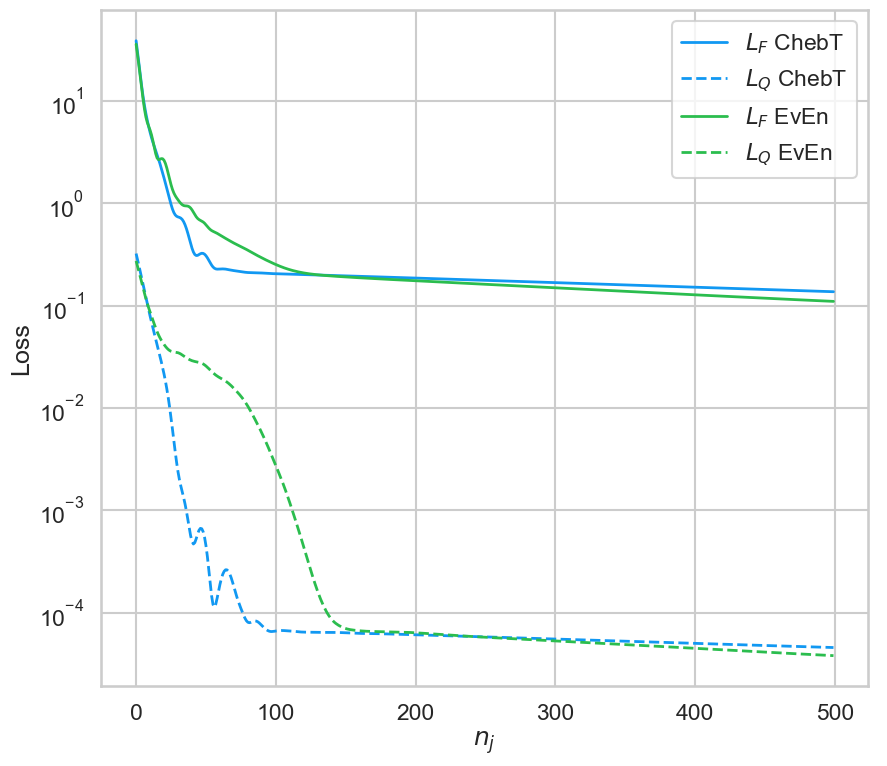
\includegraphics[width=\textwidth]{dqc-results-3-1.png}
            \caption{\textbf{Graph of Loss function over Iterations}\\
            Full loss $L_F$ is shown as solid lines, quality $L_Q$ as dashed lines.}
            \label{fig:dqc-results-3-1}
        \end{subfigure}
        \hfill
        \begin{subfigure}[t]{0.45\textwidth}
            \centering
            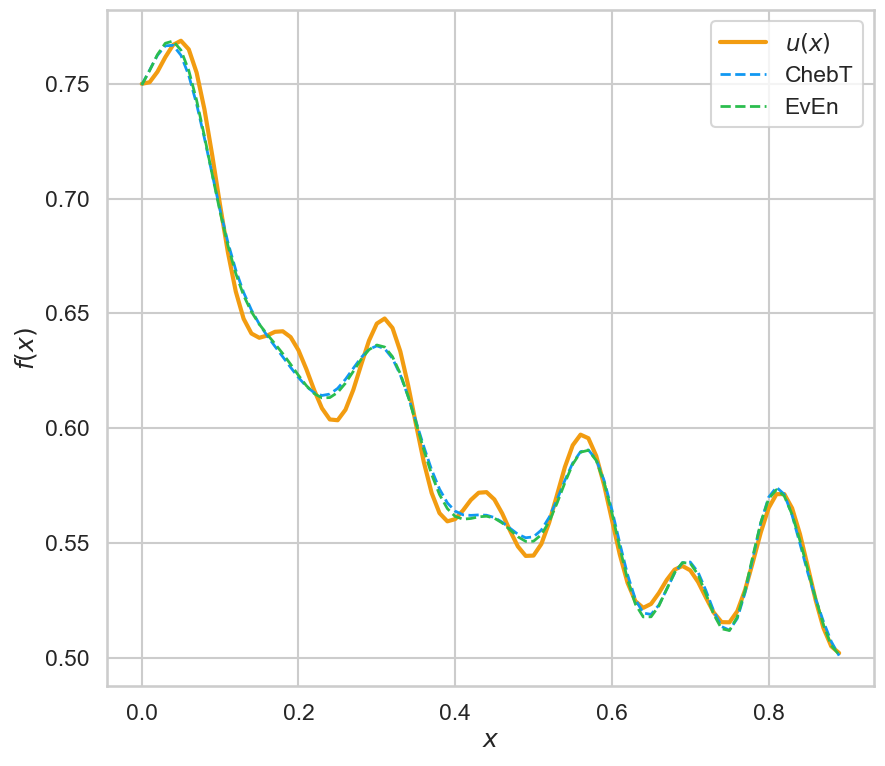
\includegraphics[width=\textwidth]{dqc-results-3-2.png}
            \caption{\textbf{Graph of corresponding trained solutions alongside known solution (shown as solid line)}}
            \label{fig:dqc-results-3-2}
        \end{subfigure}
    }
    \caption{\textbf{Results of DQC solver implemented for eq. \ref{eq:second}}}
    Chebyshev tower map (\texttt{ChebT}) is shown in blue, and evolution enhanced map (\texttt{EvEn}) is shown in green.
    \label{fig:dqc-results-3}
\end{figure}
The loss decay observed in fig. \ref{fig:dqc-results-3-1} is sharper and plateaus quickly around 150 iterations due to the less expressive ansatz structure with $d=6$ which is not able to match the complex features.
We observe that the \texttt{Even} map shows poor optimization in the first 150 iterations, owing to the complex state space produced by the Hamiltonian time evolution but improves later, and converges to a better solution. This is expected since it introduces entangled states in the model which increase expressibility.
However, the improvement is not significant which indicates further optimization is required in regard to choice of Hamiltonian and time constant $\tau$.

\subsection{Application - 2D Laplace Equation}

Many industrial and scientific problems are described as partial differential equations (PDEs), and finding their solutions is the focus of numerous classical numerical and physics-informed deep learning methods.

As a final demonstration of the DQC solver workflow, we attempt to solve the Laplace equation in two spatial dimensions given by the differential equation

$$
\frac{\partial ^2 u}{\partial x^2} + \frac{\partial ^2 u}{\partial y^2} = 0
$$

\begin{figure}[H]
    \centering
    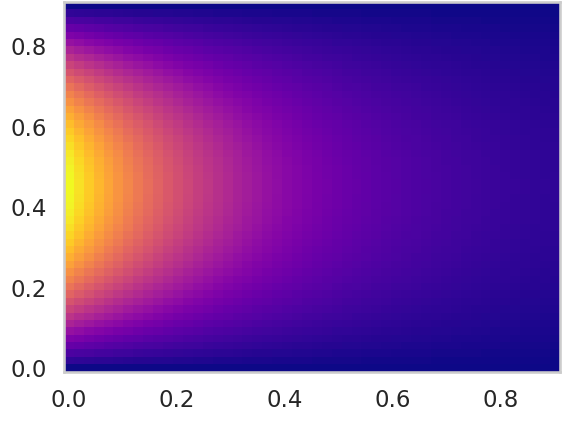
\includegraphics[width=0.6\textwidth]{laplace-solution.png}
    \caption{\justifying\textbf{Graph of the known analytical solution to the 2D Laplace equation:} $u(x,y) = e^{- \pi x} \sin(\pi y)$}
    \label{fig:laplace-solution}
\end{figure}

We aim to train the model to approximate the known exact solution $u(x,y) = e^{-\pi x} \sin(\pi y)$ in the domain $(x, y) \in \Omega = [0, 1] \times [0, 1]$, using the Dirichlet boundary conditions for $(x, y) \in \Gamma = \partial\Omega$ given as:

\begin{align*}
    u(0,y) &= \sin(\pi y) \\
    u(x,0) &= 0 \\
    u(1,y) &= e^{-\pi} \sin(\pi y) \\
    u(x,1) &= 0
\end{align*}

\subsection{Hard constraint-based physics informed neural networks (hPINNs)} 

Solving the 2D Laplace equation is key to many physics-based PDE problems, which has lead to the development of special techniques for solving them using physics-informed neural networks (PINNs).

To model the solution, we apply methods from the hard-constraint-based quantum PINN (hqPINN) framework highlighted in \cite{PINN}. We adopt the technique of using a model architecture that enforces hard boundary constraints, allowing the neural network specifically focus on minimizing the PDE residual only, specifically for the case Dirichlet boundary conditions as described above.

An exact model architecture suggested in \cite[p.~5]{HQNN} is considered. We extend this technique to the two dimensional Dirichlet boundary condition case. First we split the boundary into four intervals defined as $\{x = 0, 0\leq y\leq 1\}, \{0\leq x \leq 1, y = 0\}, \{x = 1, 0\leq y\leq 1\}$ and  $\{0\leq x \leq 1, y =1\}$, indexed 1 through 4 for brevity. For every point $(x,y) \in \Omega$, define $d_i = d_i(x,y), \;i \in \{1,2,3,4\}$ as the distance from the $i$-th boundary and $c_i = c_i(x,y), \; i \in \{1,2,3,4\}$ as the boundary value at the point corresponding perpendicular projection of the general point on the $i$-th boundary interval.

We define the (hqPINN) trial function as:
$$
f_{\varphi,\boldsymbol{\theta}}(x,y)_{\text{hqPINN}} = \sum_{\text{cyclic } i,j,k,l} c_{i} e^{-k d_{i}} (1 - e^{-k d_{j}}) (1 - e^{-k d_{k}}) (1 - e^{-k d_{l}}) + \braket{\mathcal{\hat{U}}_{\varphi,\boldsymbol{\theta}}(x,y)} \;\prod_i (1 - e^{-k d_{i}})
$$
For $i,j,k,l$ cycling through $\{1,2,3,3\}$ resp., with $\braket{\mathcal{\hat{U}}_{\varphi,\boldsymbol{\theta}}(x,y)}$ being the output from the quantum neural network and $k \in \mathbb{R}$ is a hyperparameter.
This ensures that the network is constrained towards the boundary values when the points lie very close to the boundaries, and the contribution of the constraint decays exponentially as the point moves perpendicularly away from the corresponding boundary.

This offers another inherent advantage to the solver in this specific case; the exponential decay term matches the $ e^{-\pi x}$ term in the true solution very well, allowing easier training of the model. This can be seen in the output of an untrained, randomly initialized model in \ref{fig:hqpinn-init} initialized with \texttt{torch.manual\_seed(4)}.

\begin{figure}[H]
    \centering
    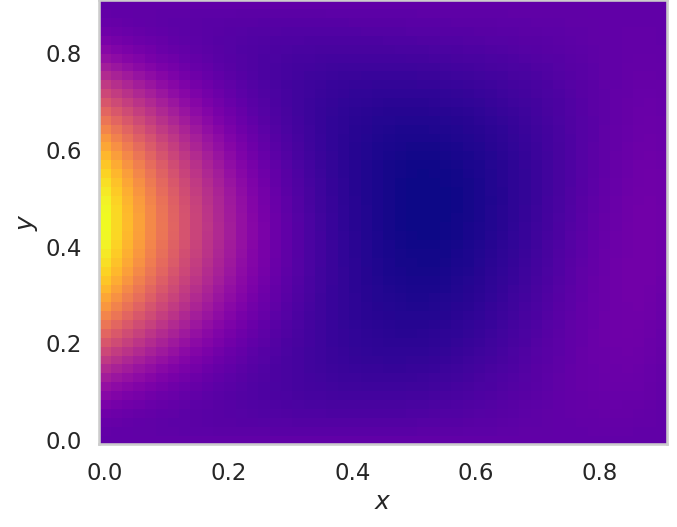
\includegraphics[width=0.6\textwidth]{hqpinn-init.png}
    \caption{\justifying\textbf{Graph of the output from an untrained hqPINN model:} $k = 1.5$ is used and parameters are randomly initialized in $[0, 2\pi / 10)$}
    \label{fig:hqpinn-init}
\end{figure}

\subsection{Methodology - 2D Laplace equation (using hqPINN)}

\begin{figure}[H]
    \centering
    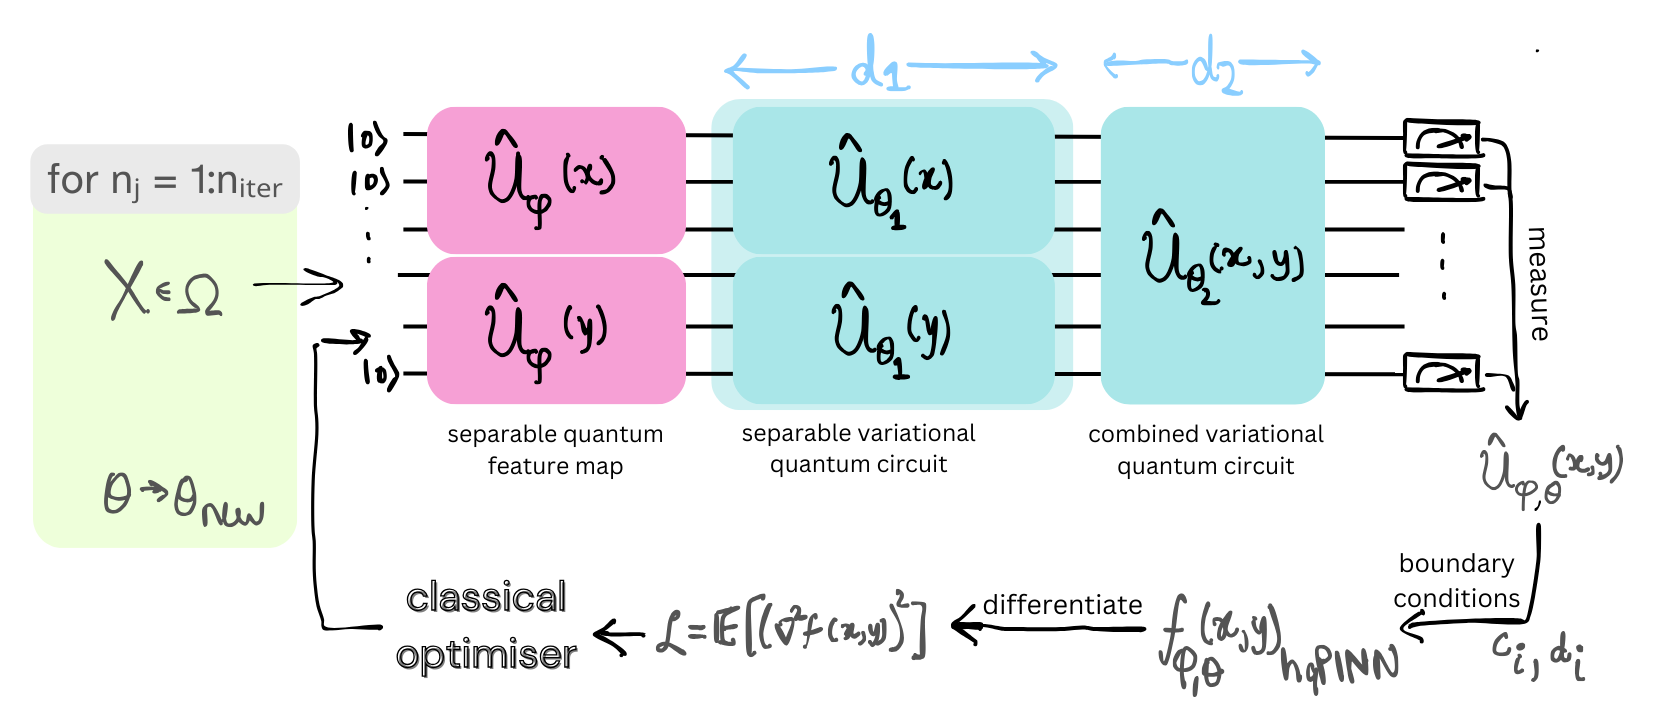
\includegraphics[width=\textwidth]{hqPINN-schematic.png}
    \caption{\justifying\textbf{hqPINN model schematic:}
    hqPINN model can be viewed as two independent QNNs trained to represent features in domains of variables $x$ and $y$ seperately, followed by variational combining of the results which are then extracted as a single trial function $f(x)$, by combining with classically processed boundary condition-based parameters $c_i, d_i$, which is then differentiated to compute loss, followed by a classical optimization loop, repeated for $n_{\text{iter}}$ iterations.}
    \label{fig:hqpinn-schematic}
\end{figure}

\vspace{1.5em}

We use the same basic workflow outline as described and implemented in above sections, and describe the major changes made in the methodology in this section.

We can breakdown the task of extending our solver to a 2D PDE as:

\begin{enumerate}
    \item \textbf{Problem definition:} The PDE is generated by taking second order derivatives by applying \texttt{torch.autograd.grad} method twice recursively and extracting the double partial derivatives with respect to $x$ and $y$.

    \item \textbf{Quantum feature map:} To map the vector $(x, y)$ to a suitable expressive function space using $N$ qubits, we use the Kronecker product of two seperate $N / 2$ qubit Chebyshev tower maps applied over complementary set of qubits. This is used because the solution is seperable in the two variables as $u(x,y) = f(x) g(y)$ so the features in both domains can be seperately trained to high accuracy.

    \item \textbf{Ansatz structure:} Inspired by the same line of reasoning, we use a moderate depth $d_1$ ansatz ($\mathcal{\hat{U}}_{\boldsymbol{\theta_1}}(x,y)$) which consists of two blocks of HEA applied over the $x$ and $y$ feature mapped qubits seperately, followed by a low depth $d_2$ ansatz ($\mathcal{\hat{U}}_{\boldsymbol{\theta_2}}(x,y)$) which consists of single HEA block applied over the entire qubit set. This structure allows the solver to optimize the parameters $\boldsymbol{\theta_1}$ corresponding to features in both variables seperately. Then, the second ansatz $\mathcal{\hat{U}}_{\boldsymbol{\theta_2}}(x,y)$ introduces global entangling behaviour which adds the capability to represent mixed behaviour (non-seperable into $x$ and $y$ components) which can increase expressibility.

    \item \textbf{Loss function:} We use the physics-informed loss function, that also corresponds to the PDE residual, that is, squared value of the Laplacian averaged over the training grid.
    $$
    \mathcal{L}_{\text{hqPINN}} = \frac{1}{M} \sum_{i=1}^{M} (\nabla^2 f_{\varphi,\boldsymbol{\theta}}(\boldsymbol{x_i})_{\text{hqPINN}})^2
    $$
    where $\{\boldsymbol{x_i}\}_{i=1}^{M}$ is the training grid.
    The boundary loss term is not considered since we are using a hqPINN model.

    \item \textbf{Optimizer:} We use the Adam optimizer with a learning rate \\ scheduler (using \texttt{torch.optim.lr\_scheduler.ReduceLROnPlateau}).
    
\end{enumerate}

\subsection{Analysis}
We report and analyze the results obtained for various setups of the hqPINN-based DQC solver. $N=6$ qubits are used (sufficiently expressible to approximate the simple features separately) and the model is trained on a uniformly spaced grid of $50 \times 50$ points. Learning rate used is 0.01 and the scheduler uses patience of 10 epochs, reduction factor of 0.5 and minimum bound on learning rate set as $10^{-5}$. The model is trained for 500 epochs. Training time \footnote{All experiments were conducted on a laptop equipped with an NVIDIA GeForce RTX 4050 (Laptop GPU, 6GB VRAM), an AMD Ryzen 7 7840HS CPU, and 16GB RAM.} and final solution quality are presented in \ref{fig:hqpinn-result-quality}.

\begin{figure}[H]
    \centering
    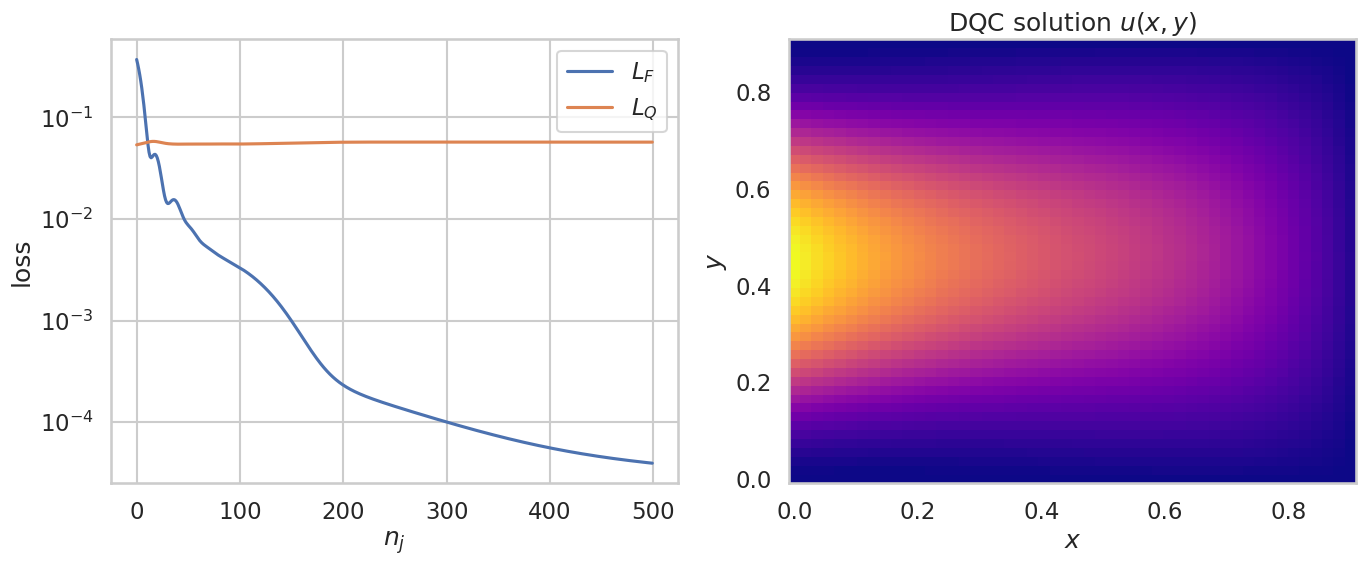
\includegraphics[width=\textwidth]{hqpinn-result-1.png}
    \caption{\justifying hqPINN-based DQC Result for setup with $d_1=6,\; d_2=1,\; k = 1.5$ used as reference}
    \label{fig:hqpinn-result-1}
\end{figure}
\begin{figure}[H]
    \centering
    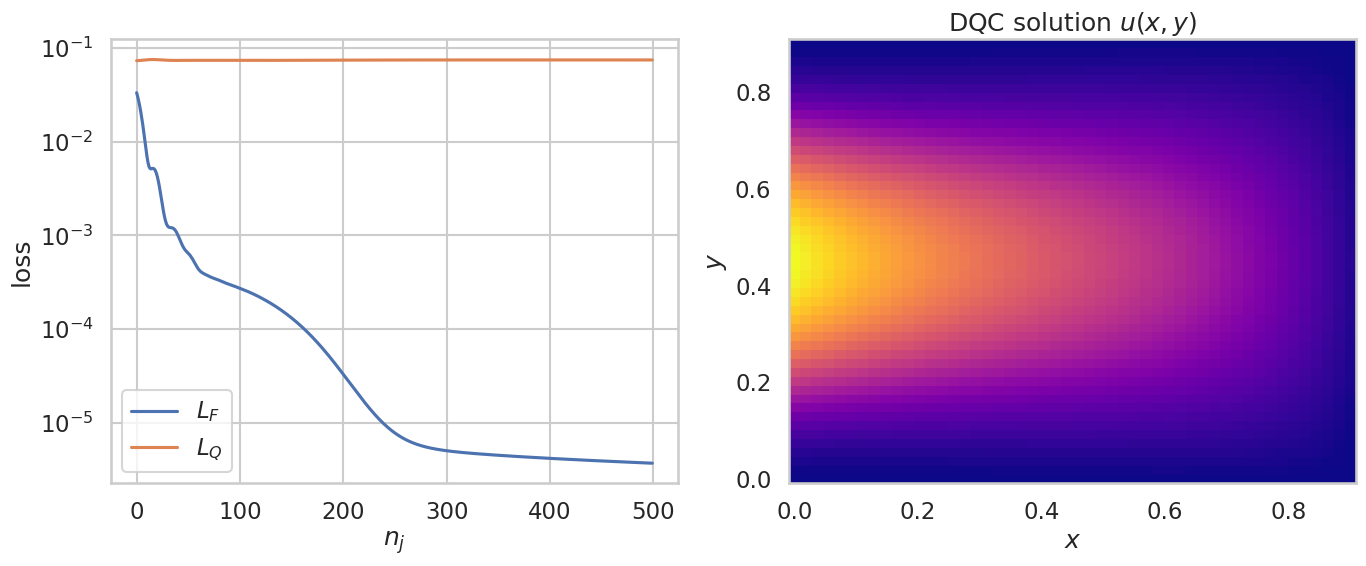
\includegraphics[width=\textwidth]{hqpinn-result-2.png}
    \caption{\justifying hqPINN-based DQC Result for setup with $d_1=6,\; d_2=1,\; k = 1.0$ to observe effect of lowering $k$ to improve optimization.}
    \label{fig:hqpinn-result-2}
\end{figure}
\begin{figure}[H]
    \centering
    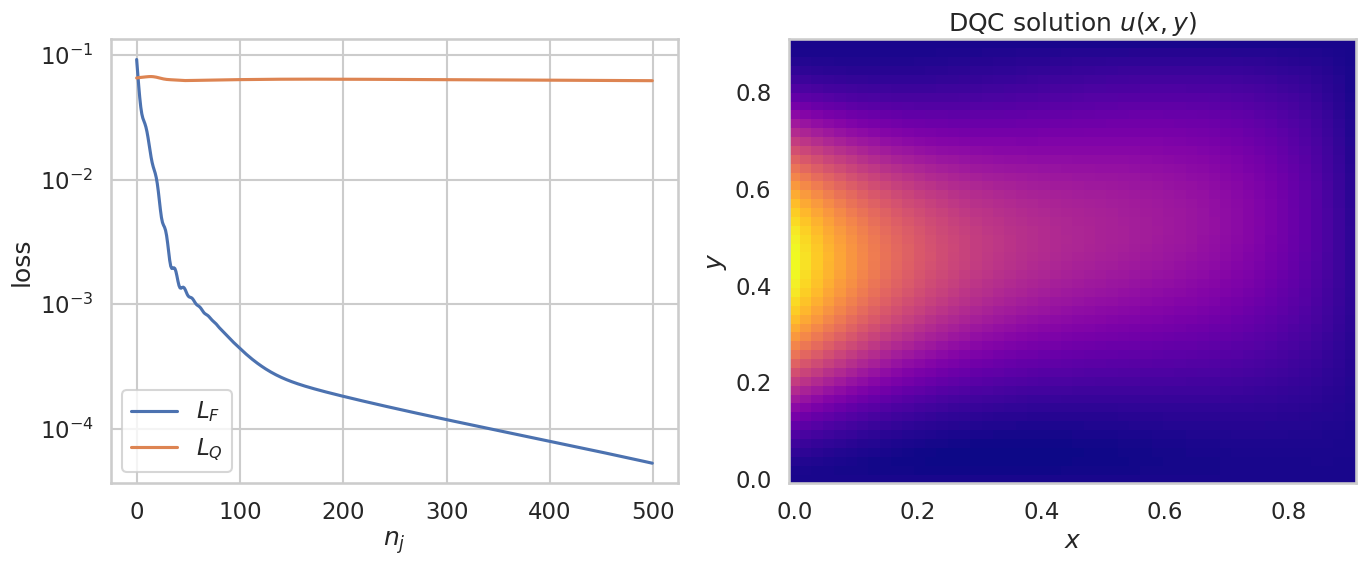
\includegraphics[width=\textwidth]{hqpinn-result-3.png}
    \caption{\justifying hqPINN-based DQC Result for setup with $d_1=6,\; d_2=4,\; k = 1.5$ to observe effect of increasing $d_2$ to provide small increase in expressibility}
    \label{fig:hqpinn-result-3}
\end{figure}
\begin{figure}[H]
    \centering
    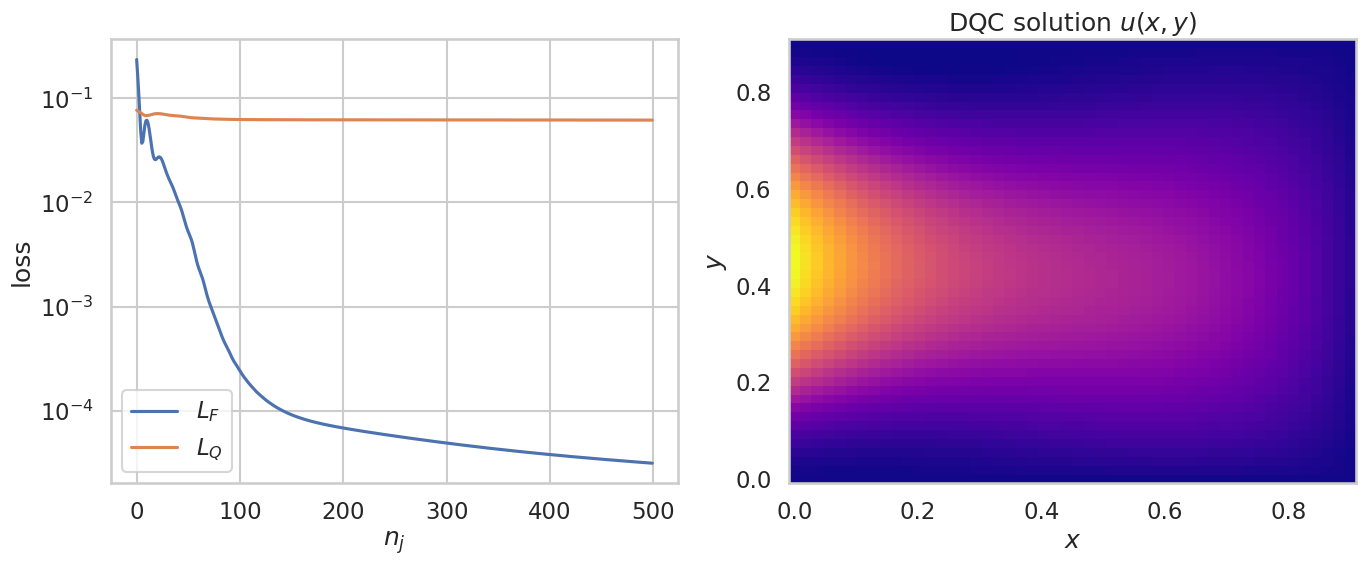
\includegraphics[width=\textwidth]{hqpinn-result-4.png}
    \caption{\justifying hqPINN-based DQC Result for setup with $d_1=9,\; d_2=1,\; k = 1.5$ to observe effect of increasing $d_1$ to provide appreciable increase in expressibility}
    \label{fig:hqpinn-result-4}
\end{figure}

\begin{figure}[H]
    \centering
    \begin{tabular}{@{}llllll@{}}
        \toprule
        Model No.  & $d_1$ & $d_2$ & $k$ & Final solution quality & Training Time \\ \midrule
        1. & 6 & 1 & 1.5 & 0.057 & 24 min.\\
        2. & 6 & 1 & 1.0 & 0.074 & 15 min.\\
        3. & 6 & 4 & 1.5 & 0.062 & 19 min.\\
        4. & 9 & 1 & 1.5 & 0.061 & 20 min.\\
        \bottomrule
    \end{tabular}
    \caption{Final solution quality obtained for various setups of the hqPINN-based DQC solver}
    \label{fig:hqpinn-result-quality}
\end{figure}


Results of the hqPINN-based DQC solver are shown for different sets of hyperparameters. Graph of loss function over iterations (left) shows full loss $L_F$ in blue and quality of solution $L_Q$ in orange. Predicted solution (right) is shown as a heatmap.\\

\begin{enumerate}
    \item The setup with $d_1=6,\; d_2=1,\; k = 1.5$ is used as reference shown in fig. \ref{fig:hqpinn-result-1}. We observe a steady loss decay similar to earlier implementations of the DQC solver. Notice that the quality loss $L_Q$ varies at a much smaller rate than $L_F$. Nonetheless, the decay is gradual which can be attributed to the fact that the untrained model matches the desired solution very well (shown in \ref{fig:hqpinn-init}) making it harder to further optimize.
    \item The setup with $d_1=6,\; d_2=1,\; k = 1.0$ is shown in fig. \ref{fig:hqpinn-result-2}. The lower value of $k$ reduces the rate of exponential decay making the model output approximate the trial function more closely hence improving optimization. However an untrained model with $k = 1.0$ shows poorer quality of solution than $k = 1.5$ (used in reference). The results are in accordance with this, as the model shows faster $L_F$ decay but slightly poorer score due to a worse solution quality at initialization.
    \item The setup with $d_1=6,\; d_2=4,\; k = 1.5$ is shown in fig. \ref{fig:hqpinn-result-3}. We expect a minor improvement in expressibility due to higher $d_2$ but at higher training cost, since the function lacks non-separable features. The results agree with it as initial $L_F$ decay is faster but finally achieves a value closer to the reference setup, and marginally worse solution quality.
    \item The setup with $d_1=9,\; d_2=1,\; k = 1.5$ is shown in fig. \ref{fig:hqpinn-result-4}. We expect a decent improvement in expressibility due to higher $d_1$ albeit at higher training cost. The results agree with it as initial $L_F$ decay is the fastest and finally achieves a value marginally smaller the reference setup although the solution quality is marginally worse.
\end{enumerate}

\subsection{Summary}
We have applied concepts related to the class of variational quantum algorithms along with methods for approximating global solutions of DEs using the idea of mapping to a latent space of rich basis set such as the Chebyshev basis set, which allows capturing highly nonlinear behaviors with fewer computational resources compared to classical methods. Moreover, we have implemented model design ideas from physics-inspired neural network (PINN) theory.

The results and analyses presented in above subsections points to the fact that this approach is practical and can be used to solve various ODEs as well as 2D PDEs. The solver can hence be realized using shallow quantum circuits with few qubits which offers scope for execution on present era quantum hardware.

The tools offered by the Qadence library can be used to explore future iterations of this approach. We can further explore implementing floating boundary handling and applying the model to larger and more complex set of PDEs like special cases of the Navier-Stokes equations. Additionally, looking at the potential uses of PINNs, we can apply the solver workflow for inverse problems from physics-heavy domains.

Overall, we conclude that DQCs offer a strong alternative to classical DE solvers, in the near-term quantum devices, and with future iterations and access to more powerful quantum hardware, they can pave the way to solving potentially intractable systems of equations which has huge applications in various fields.

\section{Conclusion}

This study begins by exploring foundational concepts in quantum mechanics and quantum computing, leveraging IBMQ hardware to solve introductory quantum mechanical problems and establish a practical understanding of quantum mechanics and basic quantum algorithms. The class of algorithms referred to as variational quantum algorithms (VQAs) is introduced as the quantum analogue to the highly successful class of convolutional neural networks (CNNs) in the field of ML. Introductory experiments demonstrated the effectiveness of the Variational Quantum Eigensolver (VQE) in calculating ground-state energies of molecular systems modelled by simple Hamiltonians, providing a clear example of how variational methods can bridge theoretical and practical approaches. These initial efforts laid the groundwork for extending quantum computational techniques to more complex applications, such as nonlinear differential equations.

Building on this foundation, we implemented Differentiable Quantum Circuits (DQCs) to solve differential equations with highly nonlinear solutions. Through advanced quantum feature maps, hybrid quantum-classical optimization, and variational ansatz designs, the study validated the ability of Chebyshev quantum feature maps and evolution-enhanced encodings to handle oscillatoric and decaying solutions effectively. We obtained useful findings regarding the trade-off between feature map and ansatz expressivity and convergence speed, emphasizing that more expressive maps like the Chebyshev Tower, and higher depth ansatzes, improve solution accuracy at the cost of computational time. Further ideas borrowed from PINN theory are used to develop a variation to solve the 2D Laplace equation. The results highlight the advantages of automatic differentiation in quantum circuits, which avoids the errors of finite-difference methods and efficiently utilizes NISQ-era hardware.

Further recommendations include:

\begin{enumerate}
    \item \textbf{Hardware-Aware Optimization}: Implement depth-optimized circuits to reduce noise impact while maintaining high expressivity. Strategies such as sparse Chebyshev maps combined with low-depth ansatz could balance performance and feasibility on current quantum devices.
    \item \textbf{Improved Loss Function Strategies}: Explore hybrid loss functions that combine mean square error with physical constraints to ensure faster convergence. Incorporating domain-specific priors via regularization could enhance solution fidelity.
    \item \textbf{Parallelism in Quantum Registers}: Expand the solver’s scalability by encoding multiple differential equations in separate quantum registers to improve optimization efficiency and exploit parallelism.
    \item \textbf{Real-Device Implementation}: Conduct experiments on state-of-the-art quantum hardware to assess robustness under noise and decoherence. Error mitigation techniques are needed to bridge gaps between simulation and implementation.
    \item \textbf{Applications in other Domains}: Extend these frameworks to coupled systems like multiphase flows, climate modeling, or biochemical reaction networks, where nonlinear PDEs are prevalent.
\end{enumerate}

By addressing these areas, the methodologies presented in this report can be extended toward broader applications, advancing the utility of quantum computing in solving real-world, complex systems.

\begin{thebibliography}{1}

\bibitem{nielsen_chuang}Nielsen, M. A., \& Chuang, I. L. (2000). \textit{Quantum Computation and Quantum Information}. Cambridge University Press.
\bibitem{VQA}Cerezo, M., et al. (2021). Variational Quantum Algorithms. \textit{arXiv preprint arXiv:2012.09265}.
\bibitem{DQC}Kyriienko, O., Paine, A. E., \& Elfving, V. E. (2021). Solving Nonlinear Differential Equations with Differentiable Quantum Circuits. \textit{arXiv preprint arXiv:2011.10395}.
\bibitem{HQNN} Ghosh, A., et al. (2023) Harmonic (Quantum) Neural Networks \textit{arXiv preprint arXiv:2212.07462}
\bibitem{PINN} Lu, L., et al. (2021) PHYSICS-INFORMED NEURAL NETWORKS WITH HARD
CONSTRAINTS FOR INVERSE DESIGN \textit{arXiv preprint arXiv:2102.04626}
\end{thebibliography}

\end{document}
